\documentclass{aa}
\usepackage{graphicx}
\usepackage[colorlinks=true, allcolors=blue]{hyperref} % color all links blue
\usepackage{amsmath}
\usepackage{mathrsfs} % for \mathscr
\usepackage{cleveref}
\usepackage{booktabs}
\usepackage[english]{babel} 
\usepackage[autostyle, english = american]{csquotes}

\usepackage{fontspec}
\usepackage[nohelv,nott]{newtxtext}
\usepackage[varg]{newtxmath}

\usepackage{fancyvrb}
\setmonofont{JuliaMono}[
  Scale = MatchLowercase,
  Path = fonts/,
  Extension = .ttf ,
  UprightFont = *-Regular, % or -Light, -Regular or -Medium
]

\usepackage{mdframed} % for colored boxes
\newmdenv[
  backgroundcolor=black!5,      % Light gray background (5% black)
  %linecolor=black,             % Frame color
  linewidth=0pt,                % Thickness of the frame
  roundcorner=0pt,              % Rounded corners
  innerlinewidth=0pt,           % Thickness of the inner line
  innertopmargin=5pt,           % Top padding
  innerbottommargin=5pt,        % Bottom padding
  innerleftmargin=5pt,          % Left padding
  innerrightmargin=5pt,         % Right padding
]{codebox}

\usepackage[dvipsnames]{xcolor}
\usepackage{tikz}
\usetikzlibrary{arrows}
\usetikzlibrary{positioning}
\usetikzlibrary{arrows.meta}
\usetikzlibrary{trees}

\DeclareMathOperator{\sinc}{sinc}
\newcommand{\LCDM}{$\mathrm{\Lambda C D M}$}
\newcommand\TODO[1]{\textcolor{red}{(\textbf{TODO:} #1)}}
\newcommand\transpose[1]{#1^\mathsf{T}}
\newcommand\scrH{\mathscr{H}}
\newcommand\lmax{l_\text{max}}
\newcommand\diff[1]{\frac{\mathrm{d}{#1}}{\mathrm{d\tau}}}
\newcommand\ddiff[1]{\frac{\mathrm{d^2}{#1}}{\mathrm{d\tau^2}}}
\newcommand\dlnfdlnx{\frac{\mathrm{d} \ln f}{\mathrm{d \ln x}}}

\newcommand\el{\mathrm{e}} % electron
\newcommand\Hy{\mathrm{H}} % Hydrogen
\newcommand\He{\mathrm{He}} % Helium
\newcommand\Hesin{{\mathrm{He}_1}} % Helium singlet
\newcommand\Hetri{{\mathrm{He}_3}} % Helium triplet
\newcommand\reone{{\mathrm{re}_1}} % 1st reionization
\newcommand\retwo{{\mathrm{re}_2}} % 2nd reionization

% link arxiv papers
\newcommand{\urlref}[1]{\url{#1}}
\newcommand{\doiref}[1]{\href{https://doi.org/#1}{\tt{DOI:#1}}}
\newcommand{\eprintref}[1]{\href{https://arxiv.org/abs/#1}{\tt{arXiv:#1}}}

\title{SymBoltz.jl: a symbolic-numeric, approximation-free and differentiable linear Einstein-Boltzmann solver}
\subtitle{}
\authorrunning{H. Sletmoen}
\titlerunning{SymBoltz.jl: a symbolic-numeric, approximation-free and differentiable linear Einstein-Boltzmann solver}
\author{Herman Sletmoen}
\institute{Institute of Theoretical Astrophysics, University of Oslo, P.O.Box 1029 Blindern, N-0315 Oslo, Norway\\\email{herman.sletmoen@astro.uio.no}}
\date{Received XX / Accepted XX}
\abstract{
SymBoltz is a new Julia package that solves the linear Einstein-Boltzmann equations.
It features a symbolic-numeric interface for specifying equations, is free of approximation switching schemes and is compatible with automatic differentiation.
Cosmological models are built from replaceable physical components in a way that scales well in model space.
The modeler should simply write down their equations, and SymBoltz solves them and eliminates much of the friction in the process.
SymBoltz enables up to $100\times$ shorter model definitions compared to browsing equivalent files in CLASS.
Symbolic knowledge enables powerful automation of tasks, such as separating computational stages like the background and perturbations, generating the Jacobian matrix and its sparsity pattern, and interpolating arbitrary expressions from the solution.
Modern implicit solvers integrate the full stiff equations at all times, reducing slowdowns by taking long time steps, reusing the Jacobian and LU-factorizing it over several time steps, and using fast linear system solvers.
Automatic differentiation gives exact derivatives of any output with respect to any input, which is important for gradient-based Markov chain Monte Carlo methods in large parameter spaces, training of emulators, Fisher forecasting and sensitivity analysis.
These features are useful in their own rights, but also reinforce each other in a synergy.
Results agree with established codes like CLASS and CAMB.
With more work, SymBoltz can grow into an integrated symbolic-numeric cosmological modeling environment with a large library of models that delivers differentiable output as fast as other codes.
SymBoltz is available at \url{https://github.com/hersle/SymBoltz.jl} with single-command installation and extensive documentation, and welcomes questions, suggestions and contributions.
% alternative: \usepackage{fontawesome} and \faicon{github}
}

\keywords{Cosmology - Methods: numerical}

\begin{document}

\maketitle

Cosmology is at a crossroads \citep{freedmanCosmologyCrossroads2017}.
Despite the enormous success of the \LCDM{} model in explaining many observations,
the increasing precision of modern observations are revealing tensions between theory and observations.
These suggest that the current standard model is not the ultimate truth.

On the theoretical side, this drives a search for the true cosmological model through modifications to \LCDM{} \citep{bull$L$CDMProblemsSolutions2016}.
Efficiently exploring the space of models benefits from numerical tools that are easy to modify.
Minimizing friction in the modeling process encourages relaxing model-dependent approximations, creating user-friendly interfaces and structuring codes in modular components that are easy to replace.
Some of the most important such tools in the cosmological modeling toolbox are linear Einstein-Boltzmann solvers (\enquote{Boltzmann codes}) like CAMB \citep{lewisEfficientComputationCMB2000a} and CLASS \citep{lesgourguesCosmicLinearAnisotropy2011}.

On the observational frontier, next-generation surveys like the
Square Kilometer Array \citep{dewdneySquareKilometreArray2009},
Vera C. Rubin Observatory \citep{lsstsciencecollaborationLSSTScienceBook2009},
Dark Energy Spectroscopic Instrument \citep{desicollaborationDESIExperimentPart2016},
Simon's Observatory \citep{thesimonsobservatorycollaborationSimonsObservatoryScience2019} and
Euclid \citep{euclidcollaborationEuclidOverviewEuclid2025}
promise even more precise data.
Setting models apart with upcoming data involves both theoretical model parameters and experimental nuisance parameters that live side-by-side in large $O(100)$-dimensional spaces \citep{pirasFutureCosmologicalLikelihoodbased2024}.
In high dimensions, modern Markov chain Monte Carlo methods like Hamiltonian Monte Carlo and the No-U-Turn Sampler \citep{hoffmanNoUTurnSamplerAdaptively2011} beat the traditional Metropolis-Hastings algorithm \citep{hastingsMonteCarloSampling1970}.
These methods explore parameter space more efficiently, but need both the likelihood and its derivatives with respect to parameters.
Differentiability is also increasingly important in other applications, such as forward-modeling field-level inference using simulations with initial conditions from Boltzmann solvers \citep{seljakOptimalExtractionCosmological2017}.
Automatic differentiation is a way to compute derivatives that is more accurate and can be faster than finite differences, which is an approximate and brute-force method.
A differentiable Boltzmann solver is therefore a cornerstone in the next-generation cosmological modeling toolbox.

SymBoltz is a new Boltzmann solver that aims to fill these gaps, featuring a convenient symbolic-numeric interface, approximation-freeness and differentiability.
At its core, a Boltzmann code solves the gravitational (Einstein) equations for a gravitational theory coupled to some particle species described by thermodynamic (Boltzmann) equations up to first perturbative order around a homogeneous and isotropic universe.
It can predict cosmic microwave background (CMB), baryon acoustic oscillation (BAO) or supernova (SN) observations; or be used in longer computations, such as to generate initial conditions to non-linear $N$-body simulations of large-scale structure.

This article is structured as follows.
\Cref{sec:intro} revisits the historical development of Boltzmann codes, sketches their structure, reviews methods for computing derivatives and motivates SymBoltz.
\Cref{sec:features} maps out the architecture and main features of SymBoltz and how it differs from other codes.
\Cref{sec:examples} shows some example usage.
\Cref{sec:discussion} discusses synergies and tradeoffs in the design.
\Cref{sec:conclusion} concludes with the current state of the code and future potential.
The appendices list equations, implementation details, comparison settings and testing methods.

\section{History and motivation}
\label{sec:intro}

\cite{peeblesPrimevalAdiabaticPerturbation1970} were first to numerically integrate a comprehensive set of linearized Einstein-Boltzmann equations.
Their work was refined over several years, and \cite{maCosmologicalPerturbationTheory1995} established the groundwork for modern Boltzmann solvers with their code COSMICS.
\cite{seljakLineSightApproach1996} soon realized that one can integrate photon multipoles by parts to reduce many differential equations to one integral solution and released CMBFAST.
Their \textit{line-of-sight integration} method has become a standard technique that greatly speeds up the calculation, but requires truncating the multipoles in the differential equations.
This Fortran codebase has since evolved into CAMB\footnote{\url{https://camb.info/}} written by \cite{lewisEfficientComputationCMB2000a}, which is one of the two most used and maintained Boltzmann solvers today.
\cite{doranCMBEASYObjectOriented2005} ported CMBFAST to C++ with the fork CMBEASY, which structured the code in an object-oriented fashion and improved user-friendliness, but this project is abandoned today.

\cite{lesgourguesCosmicLinearAnisotropy2011,blasCosmicLinearAnisotropy2011a} started the second major family of Boltzmann solvers with the birth of CLASS\footnote{\url{http://class-code.net}} in C.
It improved performance, user-friendliness, code flexibility, ease of modification and control over precision parameters.
It was the first cross-check of CAMB from an independent branch and boosted the scientific accuracy of the Planck mission.

Since then a healthy arms race have fueled refinements to CAMB and CLASS.
Both codes have spawned many forks for studying alternative models and performing custom calculations.
Today they are very well-made, efficient and reliable tools.

More recently, the market has seen an influx of alternative solvers that target new numerical techniques, GPU parallelization, differentiability, interactivity and symbolic computation.
\cite{refregierPyCosmoIntegratedCosmological2017a} published the first symbolic-numeric Boltzmann code PyCosmo\footnote{\url{https://pypi.org/project/PyCosmo/}}, which automatically generates efficient C++ ODE code from user-provided symbolic equations, performs sparsity optimization on its Jacobian matrix and avoids the use of approximation schemes to speed up and stabilize the integration.
\cite{hahnDISCODJDifferentiableEinsteinBoltzmann2024} published the first differentiable Boltzmann solver DISCO-EB\footnote{\url{https://github.com/ohahn/DISCO-EB}} in the JAX framework in Python, and relaxes approximation schemes to avoid complications and overhead when switching ODEs on GPUs.
Bolt.jl\footnote{\url{https://github.com/xzackli/Bolt.jl}} by \cite{liBoltjl2023} accomplishes much of the same in Julia.
SymBoltz.jl\footnote{\url{https://github.com/hersle/SymBoltz.jl}} is inspired by some of these developments.

\subsection{Structure of traditional Boltzmann solvers}
\label{sec:intro_structure}

The full Einstein-Boltzmann equations are partial differential equations
that linearize to ordinary differential equations.

In principle, the core task of a Boltzmann solver is thus very simple:
to solve these ordinary differential equations (ODEs) ${\mathrm{d}\mathbf{u}}/{\mathrm{d} \tau} = \mathbf{f}(\tau,\mathbf{u};\mathbf{p})$ for some initial conditions $\mathbf{u}(\tau_0)$ and parameters $\mathbf{p}$, including several perturbation wavenumbers, and compute desired quantities from their solution, like power spectra.

In practice, however, several properties complicate this task.
First, the equations separate into computational stages that benefit substantially from being solved sequentially for performance and stability, such as the background and perturbations stages.
It is common to solve each stage with interpolated input from the previous stage, and joining these can be cumbersome and fragment code.
Second, the set of equations is very long and convoluted.
Ideally, parts of the equations should be easily replaceable to accommodate different cosmological (sub)models.
Organizing a code with a suitable modular structure that scales well in model space is hard.
Third, tension between wildly different timescales that coexist in the equations make them extremely stiff and intractable for standard explicit ODE solvers.
This stiffness must be massaged away in the equations or dealt with numerically in other ways.
Fourth, the size of differential equations is very large and increases for more accurate description of relativistic species.
Typical models with accurate treatment of photons and neutrinos need $O(100)$ equations.
Fifth, the perturbations must be solved for many different wavenumbers $k$, and tradeoffs between performance and accuracy must be made.

To overcome these challenges, Boltzmann solvers are typically written in low-level high-performance languages like C, C++ and Fortran.
Codes are usually tightly adapted to the pipeline-like \emph{computational} structure of the problem (e.g. input $\rightarrow$ background $\rightarrow$ thermodynamics $\rightarrow$ perturbations $\rightarrow \ldots \rightarrow$ output in section 3.3 in \cite{lesgourguesCosmicLinearAnisotropy2011}).
This makes sense for the programmer and computer, but not always for the modeler.

Traditional codes have nonexistent or only very thin abstraction layers around them.
To modify them, users must work directly in the low-level numerical interface and should be prepared to get their hands dirty.
For example, to implement a new species, one must generally modify the code in many places: input handling for any new parameters, new background equations, new thermodynamics equations, new perturbation equations, joining between each of these stages, output handling, and possibly more.
This leads to fragmented code where the changes related to one species are scattered throughout the code, making it challenging and unintuitive to navigate and decipher.

More importantly, this structure scales poorly in model space.
Each module becomes more polluted as more components are added.
Even if they are deactivated by if statements at runtime, their mere presence in the source code reduces its readability.
In turn, the whole code grows into a complex and mysterious beast.

One can alleviate this problem to some extent by instead forking the code for modified models, so the main code base is not polluted.
But this just moves the problem.
Forking duplicates the entire code base even though only small parts are modified.
Forks are often abandoned and do not receive upstream improvements.
They are also incompatible with each other unless one merges them into one code, but then one is back to the first problem.

The two-language problem amplifies the problem, as data analysis usually takes place in slower high-level languages like Python.
This shapes Boltzmann solvers to rigid pipelines that must compute everything in one shot and avoid interception at all costs, in order to maximize performance in the low-level language before passing the data back to the high-level language.
Some features that are really just post-processing of the ODE solutions are appended to the pipeline even if they are peripheral to the core task of an Einstein-Boltzmann solver -- which is to solve the Einstein-Boltzmann equations.
This includes non-linear boosting and CMB lensing, for example.

These code smells lead to big monolithic \enquote{black boxes} that scale poorly in model space, and whose complexity grows to incorporate features beyond their original core scope.
This complexity has even fueled development of specialized AI assistants for CLASS \citep{casasCLAPPCLASSLLM2025}.
While such tools are helpful, we think they are a symptom of unnecessary complexity and poor scaling with the number of models.
Of course, there are also some advantages to this structure, as we discuss in \cref{sec:discussion}.

\subsection{Boltzmann solver approximation schemes}
\label{sec:intro_approximations}

The Einstein-Boltzmann equations are infamously \emph{stiff}.
This is a property of differential equations \eqref{eq:ode} that means their numerical solution is unstable and requires tiny step sizes with standard explicit Runge-Kutta methods.
Stiffness can arise when multiple and very different time scales appear in the same problem.
This is very common in cosmology, where particles interact very rapidly in a universe that expands very slowly, particularly in the tightly coupled baryon-photon fluid, for example.
Stiff equations are practically impossible to integrate with explicit solvers and require special treatment.

For a long time, Boltzmann solvers have massaged away stiffness with several approximation schemes%
\footnote{Here \enquote{approximations} refers to schemes that switch between different equations at different times. It excludes techniques like multipole truncation and line-of-sight integration, which SymBoltz also uses.}
in the equations (e.g. \cite{doranSpeedingCosmologicalBoltzmann2005,blasCosmicLinearAnisotropy2011a}):
\begin{itemize}
\item tight-coupling approximation (TCA),
\item ultra-relativistic fluid approximation (UFA),
\item radiation streaming approximation (RSA),
\item Saha approximation.
\end{itemize}
These usually involve switching from one set of equations to another when some control variable that measures the applicability of the approximation crosses a threshold.
This can change the unknowns in the ODE and require reinitializing it.
The approximations help stability and sometimes performance of the equations and allow the use of explicit solvers.

However, approximations put much more strain on the modeler to derive and validate versions of their equations in different regimes.
Furthermore, this process should generally be repeated when further changes are made to the model.
The numerics also become more complicated: timeseries from each ODE solution must be stitched together, tolerances are duplicated for each separate ODE system that may respond differently to them, ODE integrators must be reinitialized, and so on.

It is a misunderstanding in the literature that it is \enquote{difficult} or \enquote{impossible} to solve the Einstein-Boltzmann equations without using approximations, or that they are \enquote{unavoidable} \citep[][respectively]{maCosmologicalPerturbationTheory1995,lewisCAMBNotes2025,lesgourguesCosmicLinearAnisotropy2011}.
This statement must only be understood in the context of explicit solvers!
Implicit integrators can solve stiff equations, but seem largely underutilized by Boltzmann solvers, perhaps because they are scarce and harder to implement.
CLASS has an implicit solver, but does not permit disabling all approximations \cite{blasCosmicLinearAnisotropy2011a}.
On the contrary, new life has been breathed into this field recently, as development of modern implicit solvers and techniques like automatic and symbolic differentiation make implicit solvers more feasible and powerful.

\subsection{Differentiation methods}
\label{sec:intro_diff}

Derivatives are important in computing.
Cosmological applications are no exception.
For example, algorithms that optimize likelihoods and Markov chain Monte Carlo (MCMC) samplers for Bayesian parameter inference can take advantage of derivatives of the likelihood with respect to each parameter to intelligently step in a direction where the likelihood or probability increases.
In machine learning, the same applies when training neural networks emulators for cosmological observables as functions of cosmological parameters by minimizing scalar loss functions.
Some cosmologies are parametrized as boundary-value problems with the shooting method, and use nonlinear root solvers like Newton's method that need Jacobians.
Jacobians are also used by implicit ODE solvers to solve for values at the next time step.
Fisher forecasting uses the Hessian (double derivative) of the likelihood with respect to parameters to predict how strong parameter constraints that can be placed by data with given errors.
Boltzmann solvers typically save computational resources by interpolating spectra computed on coarse grids of $k$ and $l$ to finer grids, and this can be made more precise with knowledge of derivatives with respect to $k$ and $l$.
These are all examples where Boltzmann solvers or applications that use them need derivatives.

There are at least four ways to compute derivatives.
\textit{Manual differentiation} is the exact pen-and-paper method with differentiation rules, but is limited to simple expressions and by human error.
\textit{Symbolic differentiation} automates this process with computer algebra systems,
but is inherently symbolic and cannot differentiate arbitrary programs nested with control flow through conditional statements and loops that depend on numerical values.
\textit{Finite differentiation} approximates the derivative $f^\prime(x) \approx (f(x+\epsilon/2) - f(x-\epsilon/2)) \,/\, \epsilon$ with a small $\epsilon > 0$ (here using central differences) by simply evaluating the program several times.
This can differentiate arbitrary programs, but is approximate, introduces the step size $\epsilon$ as a hyperparameter that must be tuned for both accuracy and stability, and is a brute-force approach that requires $O(n)$ ($2n$ using central differences) evaluations to compute the gradient of an $n$-variate scalar $f$.
\textit{Automatic differentiation} \citep[e.g.][]{griewankEvaluatingDerivatives2008} can be understood by viewing any computer program as a (big) composite function
\begin{equation}
    \boldsymbol{f} = \boldsymbol{f}_N \circ \boldsymbol{f}_{N-1} \circ \cdots \circ \boldsymbol{f}_2 \circ \boldsymbol{f}_1 = \boldsymbol{f}_N(\boldsymbol{f}_{N-1}( \cdots \boldsymbol{f}_2(\boldsymbol{f}_1)))
\label{eq:program}
\end{equation}
of (many) elementary operations $\boldsymbol{f}_i: \mathbb{R}^{a_i} \rightarrow \mathbb{R}^{b_i}$ (think of $\boldsymbol{f}_i$ as the $i$-th line of code).
It then numerically evaluates the chain rule
\begin{equation}
    \boldsymbol{J} = \boldsymbol{J}_N \cdot \boldsymbol{J}_{N-1} \cdots \boldsymbol{J}_2 \cdot \boldsymbol{J}_1.
\label{eq:program_derivative}
\end{equation}
through the Jacobian $(\boldsymbol{J}_n)_{ij} = \partial f_{n,i} / \partial f_{n-1,j}$ of every elementary operation to accumulate the derivative of the entire program.
This is numerically exact, free of precision parameters, usually requires fewer operations than finite differences, but is perhaps less intuitive, harder to implement and needs the source code to interpret the program \eqref{eq:program} in the non-standard way \eqref{eq:program_derivative}.

Notably, while the function \eqref{eq:program} must be evaluated inside-to-outside (right-to-left),
the chain rule \eqref{eq:program_derivative} is an \emph{associative} matrix product that can be evaluated in any order.
This generally changes the number of operations and is a more open-ended computational problem.
\textit{Forward-mode} automatic differentiation seeds $\boldsymbol{J}_1 = \boldsymbol{1}$ (the derivative of the input with respect to itself) and multiplies $\boldsymbol{J}_N (\boldsymbol{J}_{N-1} (\cdots (\boldsymbol{J}_2 (\boldsymbol{J}_1))))$ by \enquote{pushing} every column of $\boldsymbol{J}_1$ forward through the product in the same evaluation order as $\boldsymbol{f}$.
\textit{Reverse-mode} first computes $\boldsymbol{f}$ in a forward pass, then seeds $\boldsymbol{J}_N = \boldsymbol{1}$ (the derivative of the output with respect to itself) and multiplies $((((\boldsymbol{J}_N) \boldsymbol{J}_{N-1}) \cdots) \boldsymbol{J}_2) \boldsymbol{J}_1$ by \enquote{pulling} every row of $\boldsymbol{J}_N$ backwards through the product.
This usually makes forward-mode faster when $\boldsymbol{f}: \mathbb{R}^a \rightarrow \mathbb{R}^b$ has more outputs $b \gg a$, and reverse-mode better when there are more inputs $a \gg b$.

In practice, both modes are implemented using techniques like operator overloading or source code transformation.
The former overloads every operation to accept a special number type that propagates both values and derivatives, such as \textit{dual numbers} for forward-mode \cite[e.g.][]{revelsForwardModeAutomaticDifferentiation2016}.
The latter transforms the code for $\boldsymbol{f}$ into another code that computes $\boldsymbol{J}$.
In any case, automatic differentiation requires access to the source code!

\begin{figure*}
    \centering
    \begin{tikzpicture}[
        remember picture, % nested nodes work better
        node distance=6.5cm,
        every node/.style = {align=center},
        wrapper/.style = {rectangle, rounded corners, fill=black!10, font=\normalsize, minimum width=4.7cm, minimum height=6.0cm},
        comp/.style = {draw, circle, fill=gray, minimum size = 1.3cm, inner sep = 0pt, font=\tiny},
        interaction/.style = {{Latex[width=1mm,length=1mm]}-{Latex[width=1mm,length=1mm]}},
        stage/.style = {draw, minimum height=1cm, minimum width = 3cm, fill=lightgray!75},
        process/.style = {-{Latex[width=2mm,length=2mm]}, very thick},
        bigprocess/.style = {-{Latex[width=4mm,length=4mm]}, very thick},
        title/.style = {anchor=north, text width=4cm, align=center, yshift=-0.15cm, font=\bfseries},
    ]
    \node (model) [wrapper] {
        \begin{tikzpicture}[remember picture, node distance=1cm]
            \node [comp, fill=black!40] (grav) {Gravity} [interaction, grow cyclic, level 1/.append style = {level distance = 1.7cm, sibling angle = 60}]
            child { node[comp, fill=blue!50] (bar) {Baryons}}
            child { node[comp, fill=magenta!50] (pho) {Photons}}
            child { node[comp, fill=red!50] (neu) {Massless\\neutrinos}}
            child { node[comp, fill=orange!50] (mneu) {Massive\\neutrinos}}
            child { node[comp, fill=LimeGreen!75] (cdm) {Cold dark\\matter}}
            child { node[comp, fill=Cyan!50] (cc) {Cosmo-\\logical\\constant}};
            \draw[interaction] (bar) -- (pho);
        \end{tikzpicture}
    };
    \node[title] at (model.north) {Symbolic model};
    \node (problem) [right of=model, wrapper] {
        \begin{tikzpicture}[font=\small, node distance=1.6cm]
            \node (bg) [stage] {Background};
            \node (pt) [stage, below of=bg] {Perturbations};
            \node (more) [stage, below of=pt] {\ldots};
            \draw [process] (bg) -- (pt);
            \draw [process] (pt) -- (more);
        \end{tikzpicture}
    };
    \node[title] at (problem.north) {Numerical problem};
    \node (solution) [right of=problem, wrapper] {
        \begin{tikzpicture}[font=\small, node distance=1.6cm]
            \node (bg) [stage] {Background};
            \node (pt) [stage, below of=bg] {Perturbations};
            \node (more) [stage, below of=pt] {\ldots};
            \draw [process] (bg) -- (pt);
            \draw [process] (pt) -- (more);
        \end{tikzpicture}
    };
    \node[title] at (solution.north) {Solution object};
    \draw [bigprocess] (model) -- node [above=1mm] {Compile} (problem);
    \draw [bigprocess] (problem) -- node [above=1mm] {Solve} (solution);
    \end{tikzpicture}
    \caption{SymBoltz represents cosmological models with equations in \emph{symbolic} form and grouped by physical components like the spacetime metric, gravity and particle species. This is compiled to a \emph{numerical} problem that splits the model into background and perturbation stages and generates efficient numerical code for ODEs and their Jacobians. The problem is then solved and the result stored in a solution object that gives convenient access to any quantity defined in the symbolic model.}
    \label{fig:components}
\end{figure*}

\section{Code architecture and main features}
\label{sec:features}

SymBoltz is built somewhat differently than other Boltzmann codes.
In short, it uses a symbolic-numeric abstraction interface where users enter high-level symbolic equations, and automatically compiles them to fast low-level numerical functions.
It cures stiffness with implicit ODE solvers, and uses no approximation schemes to keep models simple, elegant and extensible.
It is differentiable, so one can easily get accurate derivatives of any output with respect to any input.
This provides rapid model prototyping, helpful abstractions and automation of typical chores when modifying other codes.
SymBoltz encourages interactive usage and pursues a modular design that lets users integrate whatever they need from the package into their own applications.
The end goal is to prioritize the \emph{modeler}, who should be able to just write down the model equations while SymBoltz takes care of the rest.

SymBoltz is written in the Julia programming language \citep{bezansonJuliaFreshApproach2017a}, which attracts development of modern numerical methods and aims to resolve the two-language problem.
The symbolic-numeric interface is built on the ModelingToolkit.jl \citep{maModelingToolkitComposableGraph2022} and Symbolics.jl \citep{gowdaHighperformanceSymbolicnumericsMultiple2022} packages.
The compiled functions are integrated by implicit ODE solvers in DifferentialEquations.jl \citep{rackauckasDifferentialEquationsjlPerformantFeatureRich2017}.
Everything works with automatic differentiation through ForwardDiff.jl \citep{revelsForwardModeAutomaticDifferentiation2016}, for example.

The next subsections present the design of SymBoltz in more detail, revolving around the three key features in the title.
Other minor implementation details are given in \cref{sec:implementation}.
\textbf{This paper is as of SymBoltz version 0.8.1. Please refer to the package documentation for definitive up-to-date information.}

\subsection{Symbolic-numeric interface}
\label{sec:symbolicnumeric}

The core of SymBoltz is built around a symbolic-numeric interface shown in \cref{fig:components}.
Variables and equations are specified in a high-level user-friendly symbolic modeling language, then ultimately compiled down to efficient low-level numerical functions that are integrated by ODE solvers.
This fits the interactive and just-in-time compiled nature of Julia.
A key realization is that knowledge of \emph{symbolic} equations makes it possible to analyze their structure programmatically, enabling powerful transformations of the equations and automation of chores.

SymBoltz turns the layout of traditional Boltzmann solvers inside-out.
While other codes are built like rigid pipelines following \emph{computational stages} like the background and perturbations,
SymBoltz is primarily structured around \emph{physical components} of the Einstein-Boltzmann system.
Full cosmological models are built by joining submodels for the metric, gravitational theory, photons, baryons, dark matter, dark energy, neutrinos and other species.
Each component is a chunk of related variables and internal equations, and is unaware of other components.
Interactions (e.g. Compton scattering or sourcing of gravity) are equations that connect components.
This structure is made possible by the symbolic interface and would slow a purely numerical code.

Separation of computational stages is secondary and done automatically (see \cref{sec:splining}).
This makes it possible to write everything related to one component \emph{in one place}, instead of scattering code across separate modules for input, background, perturbations and so on.
One component can be replaced by another to construct a different cosmological model without polluting a big global model.
A large part of SymBoltz is thus simply devoted to building a well-organized library of such physical components.

This modular structure scales better in model space and makes it easier to assemble both extended and reduced models.
While many Boltzmann solvers hardcode baryons and photons because they are fundamental to the code, SymBoltz works naturally even with pure models with non-interacting radiation, matter and dark energy.
For example, this can help understand how a modified gravity theory responds to different species without complex interactions or thermodynamics cluttering the picture.

Maybe this structure is unfamiliar to some.
As a compromise, SymBoltz also provides an \enquote{unstructured} version of the \LCDM{} model with all equations and variables in one big system.
This makes it easy-peasy to change anything in the model, and really shows the power of the symbolic interface:
SymBoltz defines the full \LCDM{} model (with GR, baryons, RECFAST recombination, photons, cosmological constant, massive and massless neutrinos) in just 277 lines of code, while the equivalent code that one must realistically browse in CLASS is spread over 10 files with 27721 lines!%
\footnote{Counting \texttt{input.\{h,c\}}, \texttt{background.\{h,c\}}, \texttt{thermodynamics.\{h,c\}}, \texttt{perturbations.\{h,c\}} and \texttt{wrap\_recfast.\{h,c\}} with \texttt{wc -l}.}
SymBoltz has less features than CLASS, but this is not even remotely close to making up for the $100\times$ simplification.

Let us see which helpful features this interface provides.

\subsubsection{Automatic numerical code generation}
\label{sec:codegen}

SymBoltz automatically compiles symbolic equations to numerical code for ordinary differential equations (ODEs)
\begin{equation}
    \frac{\mathrm{d}\mathbf{u}}{\mathrm{d} \tau} = \mathbf{f}(\tau,\mathbf{u}).
    \label{eq:ode}
\end{equation}
The generated code is fast and prevents users unfamiliar with the language or package from writing slow numerical code.
If necessary, one can escape the standard code generation and include arbitrary numerical code, but the user is then fully responsible for its performance.
This accommodates functions that cannot be written as straightforward equations, for example if one must solve a nonlinear equation for the minimum of a potential or interpolate tabulated data.
The code generation deals with chores like dynamically allocating indices for each ODE state $u_i$, and performs optimizations such as common subexpression elimination.
This is helpful as Boltzmann solvers tend to have big $\boldsymbol{f}$, and particularly with implicit ODE solvers that call $\boldsymbol{f}$ often.

\subsubsection{Automatic handling of observed variables}
\label{sec:observed}

In general, an ODE \eqref{eq:ode} admits two types of variables: \textit{unknowns} $\mathbf{u}(\tau)$ are the variables that are integrated with respect to time, and \textit{observed} variables are functions of the unknowns.
The Einstein-Boltzmann equations are commonly formulated with many observed variables.

For example, consider the metric and gravity equations in \cref{sec:metric,sec:gravity} sourced by some arbitrary $\rho(\tau)$, $\delta\rho(\tau,k)$ and $\Pi(\tau,k)$.
Here $a(\tau)$ and $\Phi(\tau,k)$ are the only unknown (differential) variables that the ODE solver must solve for,
while one can \enquote{observe} $z(\tau)$, $\scrH(\tau)$, $H(\tau)$, $\chi(\tau)$ and $\Psi(\tau,k)$ from the unknowns.
Of course, it is always possible to eliminate all observeds by explicitly inserting them into the equations for the unknowns.
But this kills readability, as observed variables are helpful and natural intermediate definitions that break up the system, and one may want to extract them from the solution as well.
Furthermore, modified models can change the sets of unknown and observed variables (e.g. modified gravity can change the constraint equation for $\Psi$ into a differential equation).
It is easier to compose models when variables do not have to be hardcoded as either unknown or observed.

SymBoltz reads in an entire system of equations like that defined by \cref{sec:implementation} and automatically figures out which variables are unknown and observed.
It then generates numerical code for solving the ODE for the unknowns (see \cref{sec:codegen}),
and can lazily compute any observed variable or expression thereof from the solution of the unknowns.

The bottom line is that the user can trivially use and obtain \textit{any} variable anywhere just by referring to it, whether it is unknown or observed.
In other solvers one must look up the desired expression for observed variables and recompute them manually.
This is tedious, error-prone and can tempts users to neglect parts of expressions (e.g. approximating $\Psi \approx \Phi$ by neglecting anisotropic stress).

\subsubsection{Automatic stage separation and splining of unknowns}
\label{sec:splining}

In principle, one can solve the Einstein-Boltzmann equations by integrating the entire system (i.e. background and perturbations) at the same time.
However, the system can be broken down into sequential computational stages that each depend only on those before it.
To alleviate stiffness in each stage, separate concerns by solving every equation only once (e.g. avoid recomputing the background for every perturbation mode) and to improve performance, it is common to solve the system stage-by-stage and spline variables from one stage as input to the next.

To illustrate, again consider the general relativistic equations in \cref{sec:gravity} sourced by some given $\rho(\tau)$, $\delta\rho(\tau,k)$ and $\Pi(\tau,k)$.
Clearly $\Phi(\tau,k)$ and $\Psi(\tau,k)$ depend on $a(\tau)$, but $a(\tau)$ does not depend on $\Phi(\tau,k)$ or $\Psi(\tau,k)$ (this just reflects the perturbative nature of the problem).
One can first solve for only $a(\tau)$ in the \textit{background}, then spline $a(\tau)$ and use it as input for solving for $\Phi(\tau,k)$ and $\Psi(\tau,k)$ in the \textit{perturbations}, instead of solving for all three together and repeatedly solve for $a(\tau)$ for every $k$.

SymBoltz uses the same stage separation strategy, but automates and strengthens it with its knowledge of the symbolic equations.
First, the full symbolic model is split into background and perturbation systems.
Cubic Hermite splines are then constructed for all \emph{unknown} variables (like $a(\tau)$) to pass their solution from one stage to the next.
This type of splines is perfect for interpolating ODEs, as cubic Hermite splines increase accuracy by taking both $\boldsymbol{u}(\tau)$ and $\boldsymbol{u}^\prime(\tau)$ into account, and $\boldsymbol{u}^\prime(\tau)$ is known analytically by definition \eqref{eq:ode}.
In contrast, \emph{observed} variables (like $\Psi(\tau,k)$) are computed from the (splined) unknowns because their derivatives are not known analytically.
Splining them directly would be less accurate.
Modelers can simply write down a new background variable and access it in the perturbations for free.
They can access any variable anywhere \emph{as if} solving the entire set of equations at once, while still benefiting from splining under the hood.

The separation into background and perturbation stages just reflects the perturbative structure of the linearized Einstein-Boltzmann equations, where each order depends only on those before it, and is always guaranteed.
However, they can often be broken further down: most thermodynamics (recombination) models can be separated from the background, and some variables have integral solutions (e.g. the optical depth $\kappa(\tau) = \int_{\tau_0}^\tau \kappa^\prime(\bar\tau) \mathrm{d}\bar\tau$ or line-of-sight integration) that can be computed in isolation after solving the differential equations.
Over time, SymBoltz aims to extend the automatic background-perturbation separation by automatically incorporating more or \emph{all} stages of the equations at hand.%
\footnote{All stages can in principle be identified from a directed dependency graph between variables (e.g. from the Jacobian matrix). Cycles in the graph correspond to interdependent equations that must be integrated together in one ODE system (e.g. background and perturbations). Leaves with differentiated variables correspond to integral solutions.}
This feature is a major advantage with access to the symbolic equations.

\subsubsection{Automatic solution interpolation}
\label{sec:interpolation}

SymBoltz integrates equations in conformal time $\tau$ for several given wavenumbers $k$, and stores the result in an object that wraps independent ODE solutions for the background and perturbations for every $k$.
Conveniently, this solution object can be queried for \emph{any} variable or symbolic expression
\begin{equation}
    x(\tau, k) = x(\boldsymbol{u}(\tau, k_i)).
\end{equation}
at any $\tau$ and $k$.
The solution object automatically expands $x$ in terms of unknowns $\boldsymbol{u}$ (if $x$ is observed), and interpolates between solved wavenumbers $k_i$ (if $x$ is perturbative) and in $\tau$ using the ODE solver's built-in interpolation method (or as in \cref{sec:splining} if $x$ is splined).
This provides the modeler easy access to any variable and expression defined in the model.
The solution interpolation is also incorporated into convenient plot recipes for trivial visualization of any expressions for any $\tau$ and $k$.

\subsubsection{Automatic Jacobian generation and sparsity detection}
\label{sec:jacobian}

Just like SymBoltz generates code for $\boldsymbol{f}$ in the ODE \eqref{eq:ode}, it can use the same symbolic equations to generate its Jacobian
\begin{equation}
    J_{ij} = \frac{\partial f_i}{\partial u_j}.
\label{eq:jacobian}
\end{equation}
Jacobians are \emph{crucial} for solving stiff ODEs accurately and efficiently with implicit solvers (see \cref{sec:approx-free})!
Manually coding them is an extremely tiresome and error-prone undertaking that must be repeated for model modifications.
Evaluating them numerically with finite differences is approximate and expensive.
Automation of this procedure is a powerful feature that again enables the modeler to focus solely on the main equations.

Another benefit is that analytical knowledge of the Jacobian lets one find its exact sparsity pattern.
Numerical approaches to this are less robust and can mistake local zeros for global zeros.
This permits constant factorization of sparse Jacobians, which improves performance of implicit solvers (see \cref{sec:approx-free}).
Full support for sparse Jacobians is still ongoing work, however.

SymBoltz can fall back from symbolic to automatic differentiation for the Jacobian.
Finite differences can also be used.

\subsubsection{Automatic change of variable (future work)}
\label{sec:changeivar}

SymBoltz consistently formulates all differential equations with respect to conformal time $\tau$ as the independent variable.
This is perhaps the most common parametrization in the literature.
It is very natural because the equations are autonomous with respect to $\tau$ (i.e. $f(\tau,\boldsymbol{u}) \rightarrow f(\boldsymbol{u})$, except some multipole truncation schemes that use $1/(k\tau)$, but these are unphysical).

Some other codes inconsistently use different independent variables in different stages.
This requires manual translation into cosmic time $t$, redshift $z$, scale factor $a$ or its logarithm $b = \log a$, for example,
involving differential transformations like $\mathrm{d}t = a(\tau) \, \mathrm{d}\tau$, $\mathrm{d}z = -(a^\prime(\tau)/a(\tau)^2) \, \mathrm{d}\tau$, $\mathrm{d}a=a^\prime(\tau)\,\mathrm{d}\tau$ and $\mathrm{d}b = (a^\prime(\tau)/a(\tau))\,\mathrm{d}\tau$.
This is another mechanical and error-prone process.

In the future, SymBoltz could automate change to another independent variable (which should be one-to-one with $\tau$) by transforming the symbolic expressions.
This can be particularly useful to compute observables as a direct function of redshift, although one can invert $z(\tau)$.
This is common in fits to observations.

\subsubsection{Automatic unit handling (future work)}
\label{sec:units}

Most variables in SymBoltz are defined in internal dimensionless units (see \cref{sec:implementation}).
In the future, SymBoltz could use its symbolic pre-processing for more powerful unit features.
For example, equations could be checked for dimensional validity to catch modeling mistakes.
Input quantities could be automatically transformed from the user's preferred (dimensionful) units (e.g. $\text{Mpc}$) to internal (dimensionless) units, and then back to the user's units for output.

\subsubsection{Automatic gauge transformation (future work)}
\label{sec:gauges}

SymBoltz is currently formulated only in the conformal Newtonian gauge.
In the future, SymBoltz could conveniently transform the symbolic equations to other gauges automatically, such as the synchronous gauge used in CAMB and CLASS.

\subsubsection{Automatic initial conditions (future work)}
\label{sec:ics}

SymBoltz currently uses adiabatic initial conditions for the perturbations.
In the future, SymBoltz could generate initial conditions for arbitrary models from the equations.
This typically involves mechanical procedures like perturbation theory or power series expansion that could be automated.

\subsubsection{Automatic approximation schemes (future work)}
\label{sec:approximations}

SymBoltz is initially designed to be free of approximation schemes (see \cref{sec:approx-free}).
In the future, SymBoltz could provide convenience utilities to help derive approximations to the equations.
For example, it could automatically expand equations in power series of some smallness parameter.
This could accelerate derivation of approximations for modified models to improve their performance with less effort.

\subsection{Approximation-freeness}
\label{sec:approx-free}

SymBoltz treats stiffness in the Einstein-Boltzmann equations with modern implicit ODE solvers that integrate the full equations at all times.
It is therefore free of approximation schemes, such as the TCA, UFA, RSA and Saha approximation.
This is much friendlier to the modeler, who now simply has to provide a single set of equations instead of deriving approximations, validating them and dealing with related chores.

However, implicit ODE solvers are more expensive than explicit methods.
In particular, at every time step they must solve a nonlinear system of equations for the next unknowns.
This is usually done with Newton's method that requires the Jacobian of the nonlinear system, which in turn involves the ODE Jacobian \eqref{eq:jacobian}.
Automatic, accurate and efficient computation of the Jacobian (see \cref{sec:jacobian}) makes this less of a problem.

As the size of the ODE and its Jacobian increases (e.g. larger $\lmax$), solving the large system of equations at every time step becomes a bottleneck.
One should then transition from dense to sparse matrix methods (this is still ongoing work) and use performant matrix methods when solving the nonlinear system.
By default, SymBoltz uses the \texttt{Rodas4P} \citep{steinebachOrderreductionROWmethodsDAEs1995} solver for the background (stiff when thermodynamics is included) and \texttt{KenCarp4} \citep{kennedyAdditiveRungeKutta2003} for the perturbations.
These are both implicit solvers from DifferentialEquations.jl.
We discuss this aspect further in \cref{sec:discussion}.

In the long run, SymBoltz could also implement approximation schemes to maximize speed (see \cref{sec:approximations}).
However, the goal is to keep the code primarily approximation-free and for all approximations to be secondary and optional.

\subsection{Differentiability}
\label{sec:diff}

SymBoltz is compatible with automatic differentiation.
One can obtain the derivative of any output quantity, such as all ODE variables and derived spectra, with respect to any combination of input parameters, like the reduced Hubble parameter $h$ or cold dark matter density parameter $\Omega_{c0}$.
Automatic differentiation is also used several places internally, such as for computing the Jacobian for implicit ODE solvers (as an alternative to the fully symbolic approach) and in the shooting method (which is a nonlinear equation solver that wraps around the ODE solver).

Currently SymBoltz is only well-tested with forward-mode dual numbers through ForwardDiff.jl.
In particular, support for reverse-mode is very attractive for scalar loss applications (e.g. likelihoods), but left for future work (see \cref{sec:forwardreverse}).

\begin{figure*}
    \centering
    \includegraphics[scale=0.43]{figures/evolution.pdf}
    \caption{Included plot recipes in SymBoltz make it trivial to visualize \emph{any} symbolic variable or expression thereof from a solution of the Einstein-Boltzmann equations. This plot was made with one short line of code per subplot. Wavenumbers $k$ are in units of $H_0/c$.}
    \label{fig:output}
\end{figure*}


\section{Examples}
\label{sec:examples}

The best way to illustrate the features in \cref{sec:features} is perhaps through some examples.
The full code is as of SymBoltz version 0.8.1 and available in a notebook in the project repository.

\subsection{Basic usage workflow}

Most usage follows a model--problem--solution workflow:
\begin{codebox}
\begin{Verbatim}
using SymBoltz
M = ΛCDM(lmax = 10)
pars = Dict(
  M.γ.T₀ => 2.7, M.b.Ω₀ => 0.05, M.b.rec.Yp => 0.25,
  M.ν.Neff => 3.0, M.c.Ω₀ => 0.27, M.h.m_eV => 0.06,
  M.I.ln_As1e10 => 3.0, M.I.ns => 0.96, M.g.h => 0.7
)
prob = CosmologyProblem(M, pars)
ks = [4, 40, 400, 4000] # k / (H₀/c)
sol = solve(prob, ks)
\end{Verbatim}
\end{codebox}
The model--problem--solution split achieves three distinct goals.

First, a \textit{symbolic} representation of the \LCDM{} model \texttt{M} is created.
This is a standalone object designed to be interactively inspected and modified independently of numerics (see \cref{sec:modifying}).
It contains every variable, parameter and equation of the cosmological model structured as a graph of submodels for each logically distinct (physical) component: the metric $g$, the gravitational theory $G$, photons $\gamma$, massless neutrinos $\nu$, massive neutrinos $h$, cold dark matter $c$, baryons $b$, the cosmological constant $\Lambda$ and inflation $I$.
For example, \texttt{equations(M)} shows all model equations; \texttt{equations(M.G)} shows only the gravitational ones; \texttt{M.g.a} gives a handle to the scale factor variable $a(\tau)$ that \enquote{belongs} to the metric $g$; \texttt{M.b.Ω₀} is the density parameter $\Omega_{b0}$ in the baryon component $b$; and \texttt{parameters(M)} lists parameters of the model that the user may set.
Everything displays with \LaTeX-compatibility in notebooks to encourage interactive use.

Second, the symbolic model is compiled to a \emph{numerical} problem \texttt{prob} with parameters \texttt{pars}.
This is an expensive operation where the \enquote{magic} in \cref{sec:symbolicnumeric} happens: equations are checked for consistency and split into background and perturbation stages; observed and unknown variables are distinguished; fast ODE code is generated; background unknowns in the perturbations are replaced by splines; the Jacobian matrix is generated in numerical/analytical and dense/sparse form; and initial values are computed.
One can customize whether stages should be separated, how the Jacobian should be generated, and so on.
This is a separate step because it performs final transformations on the model \texttt{M} once the user has finished modifying and committed to it.

Third, \texttt{solve(prob, ks)} solves the background and perturbations for the requested wavenumbers \texttt{ks}.
Omitting \texttt{ks} solves only the background.
The resulting solution object \texttt{sol} provides convenient access to all model variables.
Internally, it stores the values of all ODE \textit{unknowns} at the time steps taken by the (adaptive) solvers and for every requested wavenumber.
However, it can be queried with \textit{any} time, wavenumber and symbolic expression, and will automatically compute it from the unknowns and interpolate between stored times and wavenumbers (see \cref{sec:observed,sec:splining,sec:interpolation}).
For example, calling \texttt{sol(1.0, 2.0, g.Φ+g.Ψ)} will compute $\Phi+\Psi$ at $k = 1 \, H_0/c$ and $\tau = 2 \, H_0^{-1}$ by expanding it in terms of unknowns according to the equations in \cref{sec:gravity}.
It is also possible to compute arbitrary expressions over grids of $k$ and $\tau$.
The convenient solution interface is also integrated into plot recipes for effortless visualization, as shown in \cref{fig:output}.

Other Boltzmann solvers save only a hardcoded set of variables, such as only the unknowns.
Observed variables must generally be recomputed manually, even though they are already expressed somewhere in the code.
This is cumbersome, introduces more potential for user error and adds unnecessary friction in the modeling process.
SymBoltz has higher ambitions than simply spitting out a table with some selected variables, and is designed to interactively make modifications to the model with minimal changes and easily inspect its impact on any output.

\begin{figure*}
    \centering
    \includegraphics[scale=0.43]{figures/spectra.pdf}
    \caption{Matter and CMB (TT, TE and EE) power spectra computed by SymBoltz (SB; colored lines) compared to CLASS (CL; grey dashes) with relative errors $\text{rel.err.} = P_k^\text{SB}/P_k^\text{CL}-1$ and $\text{rel.err.} = C_l^\text{SB}/C_l^\text{CL}-1$ for the $\Lambda \text{CDM}$ model. CLASS uses the precision parameters in \cref{sec:precision}.}
    \label{fig:spectra}
\end{figure*}

\subsection{Modifying models}
\label{sec:modifying}

Suppose we want to replace the cosmological constant species $\Lambda$ in the model \texttt{M} with another dark energy species.
A well-known example is dynamical $w_0 w_a$ dark energy \citep{chevallierAcceleratingUniversesScaling2001,linderExploringExpansionHistory2003} with equation of state%
\footnote{SymBoltz already includes $w_0 w_a$ as an available species.}
\begin{equation}
    w(\tau) = w_0 + w_a (1-a(\tau)).
\end{equation}
In this case, the continuity equation
\begin{equation}
    \rho^\prime(\tau) = -3\scrH(\tau)\rho(\tau)(1+w(\tau))
\end{equation}
admits the analytical solution
(by an ansatz of the same form)
\begin{equation}
    \rho(\tau)=\rho(\tau_0)a(\tau)^{-3(1+w_0+w_a)}\exp(-3w_a(1-a(\tau))).
\end{equation}
To implement this species including perturbations following \cite{putterMeasuringSpeedDark2010}, simply write down the symbolic variables, parameters, equations and initial conditions:
\begin{codebox}
\begin{Verbatim}
g, τ, k = M.g, M.τ, M.k
a, ℋ, Φ, Ψ = g.a, g.ℋ, g.Φ, g.Ψ
D = Differential(τ)
@parameters w₀ wₐ cₛ² Ω₀ ρ₀
@variables ρ(τ) P(τ) w(τ) cₐ²(τ) δ(τ,k) θ(τ,k) σ(τ,k)
eqs = [
  w ~ w₀ + wₐ*(1-a)
  ρ₀ ~ 3*Ω₀ / (8*Num(π))
  ρ ~ ρ₀ * a^(-3(1+w₀+wₐ)) * exp(-3wₐ*(1-a))
  P ~ w * ρ
  cₐ² ~ w - 1/(3ℋ) * D(w)/(1+w)
  D(δ) ~ 3ℋ*(w-cₛ²)*δ - (1+w) * (
         (1+9(ℋ/k)^2*(cₛ²-cₐ²))*θ + 3*D(Φ))
  D(θ) ~ (3cₛ²-1)*ℋ*θ + k^2*cₛ²*δ/(1+w) + k^2*Ψ
  σ ~ 0
]
initialization_eqs = [
  δ ~ -3//2 * (1+w) * Ψ
  θ ~ 1//2 * k^2*τ * Ψ
]
X = System(eqs, τ; initialization_eqs, name = :X)
\end{Verbatim}
\end{codebox}
Everything is packed down into the $w_0 w_a$ component \texttt{X}.
Note that SymBoltz encourages Unicode symbols to maximize similarity between equations and code (e.g. \texttt{Ω₀} over \texttt{Omega\_0}) and to easily display \LaTeX{} in compatible environments (e.g. notebooks).

This is all the user has to do!
Variables are automatically split into and carried across the background and perturbation stages, hooks for setting input parameters and getting arbitrary output variables are automatically available, and so on.
The modification simply consists of writing down the equations verbatim.
It could not have been more compact and to the point.

A similar modification to CLASS is more involved, for example.
It would require \emph{at least}: reading new parameters in \texttt{input.c}; declaring new background and perturbation variables in \texttt{background.h} and \texttt{perturbations.h}; solving background equations, storing desired output and coupling them to gravity in \texttt{background.c}; and recomputing or looking up background variables, solving perturbation equations and storing desired output and coupling them to gravity in \texttt{perturbations.c}.
The changes should be if-guarded correctly to ensure the code works both with and without $w_0 w_a$.

A full $w_0 w_a \text{CDM}$ model and problem can now be built by replacing the cosmological constant species \texttt{Λ} in $\Lambda \text{CDM}$ by the $w_0 w_a$ species \texttt{X}:
\begin{codebox}
\begin{Verbatim}
M = ΛCDM(Λ = X, name = :w₀wₐCDM)
pars[M.X.w₀] = -0.9
pars[M.X.wₐ] = 0.2
pars[M.X.cₛ²] = 1.0
prob = CosmologyProblem(M, pars)
\end{Verbatim}
\end{codebox}
We proceed with this new model and problem.

\subsection{Computing power spectra}

SymBoltz can compute the matter power spectrum $P(k)$ and the angular CMB power spectra $C_l^\text{TT}$, $C_l^\text{TE}$ and $C_l^\text{EE}$:
\begin{codebox}
\begin{Verbatim}
using Unitful, UnitfulAstro # for Mpc unit
ks = 10 .^ range(-4, 1, length=200) / u"Mpc"
Ps = spectrum_matter(prob, ks)
ls = 10:10:2000
Cls = spectrum_cmb([:TT, :TE, :EE], prob, ls)
\end{Verbatim}
\end{codebox}
Calling \texttt{spectrum\_matter} and \texttt{spectrum\_cmb} with \texttt{prob} will automatically select a grid of $k$ to solve the perturbations for, and interpolate between them when computing the spectra.
This is a common interpolation trick in Boltzmann solvers to integrate fewer perturbation modes.
The functions can be called with the solution \texttt{sol} instead, but will then interpolate only between the $k$ that \texttt{sol} was solved for, leaving it to the user to ensure sufficient sampling density.
\Cref{fig:spectra} shows that the spectra agree with CLASS to $1$\textperthousand{}-$1$\% or better for the chosen parameters.

\subsection{Differentiable Fisher forecasting}
\label{sec:fisher}

Fisher forecasting is a powerful technique for predicting how strong parameter constraints that can be placed by data with given errors.
It requires accurate derivatives and is a nice application for automatic differentiation.

Near a peak $\boldsymbol{\theta}_0$, where derivatives vanish, a log-likelihood function of parameters $\boldsymbol{\theta}$ is approximated by the Taylor series
\begin{equation}
    \log L(\boldsymbol{\theta}) \approx \log L(\boldsymbol{\theta}_0) - \sum_{i,j} F_{ij} (\theta_i - \bar{\theta}_i) (\theta_j - \bar{\theta}_j),
\label{eq:likelihood_expansion}
\end{equation}
where $F$ is the \textit{Fisher (information) matrix} with elements
\begin{equation}
    F_{ij} = -\frac12 \frac{\partial^2 \log L}{\partial \theta_i \, \partial \theta_j} \bigg\rvert_{\,\boldsymbol{\theta} = \boldsymbol{\theta}_0} .
\label{eq:fisher_general}
\end{equation}
Intuitively, $F$ measures how sharp the peak is, or how sensitive $\log L$ is to changes in different directions in parameter space.
Fisher forecasting is powered by the \textit{Cramér-Rao bound}, which guarantees that $F^{-1}_{ij}$ is a lower bound $\big\lvert C_{ij}\big\rvert \geq \big\lvert F^{-1}_{ij} \big\rvert$ for the covariance $C_{ij}$ between model parameters $\theta_i$ and $\theta_j$.
The inequality is more saturated the better the likelihood approximation \eqref{eq:likelihood_expansion} is (i.e. the \enquote{more Gaussian} the probability distribution is, for which the expansion is exact).
Thus, computing $F_{ij}$ at a peak and inverting it gives the tightest parameter constraints one can hope for.

Since $F_{ij}$ depends on derivatives of $\log L$, Fisher forecasting traditionally involves error-prone finite differences and step size tuning.
This problem is avoided with automatic differentiation.

To demonstrate differentiable Fisher forecasting with SymBoltz, we make the best possible CMB (TT) measurement: one of $\bar{C}_l$ over the full sky with errors only due to cosmic variance
\begin{equation}
    \sigma_l = \sqrt{\frac{2}{2l+1}} \bar{C}_l.
\label{eq:cmb_cosmic_variance}
\end{equation}
Assuming the measurements of each $\bar{C}_l$ are normally distributed and uncorrelated, the log-likelihood for this experiment is $\chi^2$:
\begin{equation}
    \log L(\boldsymbol{\theta}) = -\frac12 \sum_l \left( \frac{C_l(\boldsymbol{\theta}) - \bar{C}_l}{\sigma_l} \right)^2.
\end{equation}
In this case, the Fisher matrix \eqref{eq:fisher_general} becomes
\begin{equation}
    F_{ij} = \sum_l \frac{\partial C_l}{\partial \theta_i} \frac{1}{\sigma_l^2} \frac{\partial C_l}{\partial \theta_j} \bigg\rvert_{\,\boldsymbol{\theta} = \boldsymbol{\theta}_0},
\label{eq:fisher_special}
\end{equation}
evaluated in some fiducial cosmology $\boldsymbol{\theta} = \boldsymbol{\theta}_0$.

The derivatives $\partial C_l / \partial \theta_i$ are hard to compute and perfect candidates for automatic differentiation with ForwardDiff.jl:
\begin{codebox}
\begin{Verbatim}
using ForwardDiff: jacobian
vary = [
  M.g.h, M.c.Ω₀, M.b.Ω₀, M.b.YHe, M.ν.Neff,
  M.h.m_eV, M.X.w₀, M.X.wₐ, M.I.ln_As1e10, M.I.ns,
]
genprob = parameter_updater(prob, vary)
ls, ls′ = 100:1:1000, 100:25:1000
Cl(θ) = spectrum_cmb(:TT, genprob(θ), ls, ls′)
θ₀ = map(par -> pars[par], vary)
dCl_dθ = jacobian(Cl, θ₀)
\end{Verbatim}
\end{codebox}
Here \texttt{vary} orders the subset of parameters to differentiate with respect to, and \texttt{genprob} is a \emph{function} that generates a new problem with updated parameters \texttt{θ}.
Then \texttt{Cl} specifies a function that computes $C_l(\boldsymbol{\theta})$ for \texttt{ls}, interpolating from a coarser grid \texttt{ls′}.
This machinery just converts from SymBoltz' parameter-to-value mapping to a function of an array of parameter values, as \texttt{jacobian} requires a pure mathematical function $\boldsymbol{f}: \mathbb{R}^a \rightarrow \mathbb{R}^b$ to differentiate.
Finally $\partial C_l / \partial \theta_i$ is computed with forward-mode automatic differentiation and stored in \texttt{dCl\_dθ}, as shown in \cref{fig:derivatives}.

\begin{figure}
    \centering
    \includegraphics[scale=0.43]{figures/derivatives.pdf}
    \caption{Normalized derivatives $(\partial C_l / \partial \theta_i) / C_l$ of a CMB TT power spectrum with respect to cosmological parameters $\theta_i$ from SymBoltz and automatic differentiation (AD; colored lines) versus CLASS and central finite differences (FD; gray dashes). CLASS uses the precision parameters in \cref{sec:precision} and finite differences with $5 \%$ relative step sizes.}
    \label{fig:derivatives}
\end{figure}

\begin{figure}
    \centering
    \includegraphics[scale=0.43]{figures/forecast.pdf}
    \caption{Marginalized 68\% and 95\% 2D confidence ellipses for parameter constraints from a Fisher forecast on a cosmic variance-dominated CMB TT-only survey using the derivatives in \cref{fig:derivatives}.}
    \label{fig:forecast}
\end{figure}

It is now trivial to compute the Fisher matrix \eqref{eq:fisher_special}.
Inverting
it forecasts the constraints in \cref{fig:forecast}.
They are in excellent agreement with finite difference results from CLASS, but these required significant tuning of precision parameters and step sizes.

\subsection{Differentiable MCMC sampling with supernova data}

Finally, we show that SymBoltz can output differentiable results for gradient-based Markov chain Monte Carlo (MCMC) samplers, like the No-U-Turn Sampler (NUTS).
This state-of-the-art method uses likelihood gradients to move more intelligently in parameter space than the \enquote{blind} Metropolis-Hastings algorithm.

We predict apparent magnitudes $m(z)$ of Type Ia supernovae as a function of redshift $z$ and fit them to 1048 observations $(z_i, m_i)$ from the Pantheon dataset \citep{scolnicCompleteLightcurveSample2018}.
Such supernovae are standard candles with constant
absolute magnitude $M \approx -19.3$.
Their apparent magnitudes are $m(z) = M + \mu(z)$, where $\mu(z) = 5 \lg (d_L(z) / 10\text{ pc})$ is the distance modulus from the background-derived luminosity distance%
\footnote{This expression is valid for any $\Omega_{k0}$ with complex $\sinc(x) = \sin(x)/x$, but can be split into branches for positive, negative and zero $\Omega_{k0}$.}
\begin{equation}
    d_L(z) = \frac{c}{H_0} \frac{\chi(z)}{a(z)} \sinc \Big( H_0 \sqrt{-\Omega_{k0}} \, \chi(z) \Big) .
\end{equation}

We define the likelihood by a multivariate normal distribution of the 1048 supernovae with (constant) covariance matrix $C$ given in detail by \cite{scolnicCompleteLightcurveSample2018}.
To compute it, we interface SymBoltz with the probabilistic programming framework Turing.jl \citep{fjeldeTuringjlGeneralPurposeProbabilistic2025}, which allows a high-level description of the probabilistic model equivalent to the log-likelihood
\begin{equation}
    \log L = -\frac12 \sum_{i,j} \big(m(z_i)-m_i\big) C^{-1}_{ij} \big(m(z_j)-m_j\big) .
\end{equation}
We use the NUTS sampler in Turing.
The code for this example can be found in the paper's notebook.
For the flat $w_0 \text{CDM}$ model ($\Omega_{k0} = 0$, $w_a = 0$, fixed $\Omega_{r0}$) it gives the constraints in \cref{fig:sn}.
The results are not interesting, but show that differentiable parameter inference \emph{works} with SymBoltz.
Performance improvements are needed to make this viable also for perturbation-derived spectra.

\begin{figure}
    \centering
    \includegraphics[width=1.00\linewidth]{figures/constraints.pdf}
    \caption{Parameter inference on 1048 Type Ia supernovae from the full Pantheon supernova dataset, using 5000 MCMC samples with the gradient-based NUTS sampler in Turing.jl and differentiable theory predictions from SymBoltz.jl.}
    \label{fig:sn}
\end{figure}

\section{Discussion of design synergies and tradeoffs}
\label{sec:discussion}

A symbolic-numeric interface, lack of approximations and differentiability are interesting features in their own rights.
They also constitute a self-reinforcing synergy explained in \cref{fig:synergy}.
Like any Boltzmann solver, SymBoltz makes some tradeoffs in its design.

\begin{figure}
    \centering
        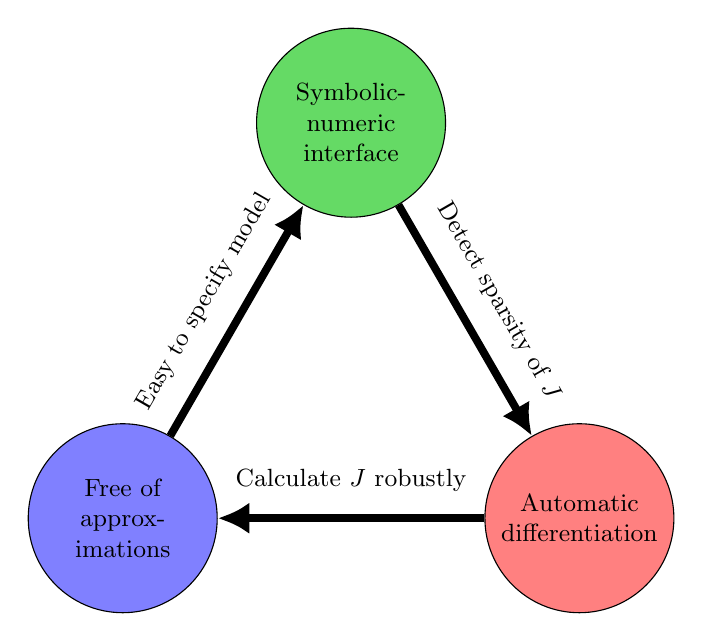
\begin{tikzpicture}[
        pillar/.style={circle, draw, minimum size=2.4cm, align=center, font=\small},
        joiner/.style={midway, sloped, black, font=\small, above, yshift=+5pt},
        arrow/.style={-{Latex[width=4mm,length=4mm]}, line width=1mm, black},
    ]
    \node[pillar, fill=LimeGreen!75] (sym) at (0:0cm) {Symbolic-\\numeric\\interface};
    \node[pillar, fill=blue!50] (app) at (240:5.8cm) {Free of\\approx-\\imations};
    \node[pillar, fill=red!50] (dif) at (300:5.8cm) {Automatic\\differentiation};
    \draw[arrow] (sym.300) -- node[joiner] {Detect sparsity of $J$} (dif.120);
    \draw[arrow] (dif.180) -- node[joiner] {Calculate $J$ robustly} (app.0);
    \draw[arrow] (app.60) -- node[joiner] {Easy to specify model} (sym.240);
    \end{tikzpicture}
    \caption{%
        A symbolic-numeric interface, approximation-freeness and differentiability are three important features of SymBoltz that form a synergy.
        For example: automatic differentiation helps to calculate the ODE Jacobian robustly; which is needed by implicit solvers to integrate stiff ODEs without approximations; which makes it easier to write down models in a simple symbolic form; which can be used to detect the sparsity pattern of the Jacobian; which in turn increases the efficiency of the implicit ODE solver.
        This synergy creates a self-reinforcing design.
    }
    \label{fig:synergy}
\end{figure}

\subsection{Symbolic vs. numeric interface}
\label{sec:symbolic_vs_numeric}

As explained in \cref{sec:intro_structure,sec:symbolicnumeric}, modifications to most Boltzmann solvers are made by editing the low-level numerical source code directly, while changes to SymBoltz are made in a high-level symbolic interface that abstracts away internal details.

We think three properties make the linearized Einstein-Boltzmann equations particularly attractive for symbolic abstraction.
First, on the \enquote{outside}, they are fundamentally \emph{one} (large) system of equations with a predictable general structure.
Second, on the \enquote{inside}, they are complicated to solve in multiple stages due to their structure, stiffness and need for speed.
Third, they are heavily subject to modifications as the true cosmological model is unknown.
To simplify the modeling process, these aspects make it valuable to abstract the \enquote{inside} from the \enquote{outside}.

Purely numerical codes generally put the \emph{programmer} first.
They are adapted to the \emph{computational} structure of the problem.
Users have full freedom to tweak problem-specific details, such as implementing complex approximation schemes.
Without abstraction layers, the code says exactly what it does.
This can be worthwhile for custom-tailoring codes to \enquote{workhorse} cosmological models like \LCDM{} for maximum performance and demanding MCMC analyses.
However, it can result in an overwhelming monolithic design that is hard to read and modify.

The symbolic interface in SymBoltz prioritizes the \emph{modeler}.
Its design matches the \emph{physical} structure of the model.
Manual chores are automated with compile-time logic on the equations.
Users can more easily change equations without understanding internals \emph{provided that} they can be written in a straightforward form that is compatible with the symbolic interface.
This is not a major restriction for the Einstein-Boltzmann equations, as they have a plain and predictable structure when linearized and free of approximations.
Nevertheless, to bridge this gap, SymBoltz lets users call arbitrary numerical functions that escape the symbolic-to-numeric compilation, if necessary.

This abstraction layer works only if fits the structure of the underlying equations.
A key to envision the design was to look past the \emph{computational} pipeline structure of Boltzmann solvers (e.g. background $\rightarrow$ perturbations $\rightarrow \ldots$), and rather organize the code primarily by \emph{physical} components like the metric, gravitational theory and particle species.
Components are self-contained and joined into full cosmological models.
As more models are added, the complexity of this modular design stays constant, while monolithic \enquote{all-in-one} codes become complicated.

This structure can be unfamiliar to those used to the layout of other codes.
The modular structure scales best with a growing number of submodels for individual physical components.
But SymBoltz also provides a full unstructured \LCDM{} model where everything is merged into one large system, which is easier to work with if one wants to modify arbitrary small parts of the equations.
This leaves the choice to the user, who can select between the best of both worlds.

Mixing symbolic and numerical computing can be susceptible to performance problems.
Numerics should be fast and symbolics is usually slow, so \enquote{perceived performance} suffers if the two are interleaved.
But SymBoltz disentangles the expensive symbolic operations in \cref{sec:symbolicnumeric} from numerics, so they are performed only before and after performance-critical tasks.

We hope the design of SymBoltz provides a platform for easy exploration of alternative models, regardless of which sector of the equations one is interested in modifying.

\subsection{Approximation-freeness vs. performance}

As seen in \cref{sec:intro_approximations}, traditional codes reduce stiffness by approximating the equations for explicit integrators,
while SymBoltz solves the full stiff system with implicit methods.

Without approximations, SymBoltz needs only one set of equations to solve.
These equations are easy to write down in pure symbolic form, which pairs nicely with SymBoltz' high-level symbolic interface.
With approximations, traditional solvers need more complicated infrastructure to switch between versions of the same equations.
This fits well to a low-level and fully numerical code that maximizes implementation freedom, like CLASS.

Approximation schemes do not only alleviate stiffness, but also improve performance by reducing the ODE size.
However, \cite{lesgourguesCosmicLinearAnisotropy2011a,hahnDISCODJDifferentiableEinsteinBoltzmann2024} found that the TCA and UFA provide only marginal speedups compared to use of implicit solvers.
On the other hand, the RSA can provide significant speedups with high $\lmax$ \citep{lesgourguesCosmicLinearAnisotropy2011a,moserSymbolicImplementationExtensions2022}.
However, more load is put on the modeler to derive, implement and validate multiple approximations.
This process must generally be repeated for modified models that can easily reintroduce stiffness or invalidate the approximations.

Implicit solvers take more expensive steps than explicit ones.
They solve a nonlinear system for the next unknowns at every time step, which gets costly as the ODE size grows (e.g. higher $\lmax$).
This is often done with Newton's method, which iterates over linear matrix solutions $A\boldsymbol{x} = b$, where $A$ involves the ODE Jacobian $J$.
But several factors mitigate this slowdown.

First and foremost, implicit solvers take longer and fewer steps due to better stability properties.
This is highly solver-dependent, however: two different implicit solvers can perform very differently on one stiff problem.
DifferentialEquations.jl lets SymBoltz easily switch between a large suite of implicit solvers.
The background (with stiff thermodynamics) is solved robustly with \texttt{Rodas4P}/\texttt{Rodas5P}, and the perturbations efficiently with \texttt{TRBDF2}/\texttt{KenCarp4}/\texttt{Rodas5P} for low/medium/high precision.
Notably, CLASS includes and defaults to a custom implicit solver \texttt{ndf15} and performs great \citep{lesgourguesCosmicLinearAnisotropy2011a}.
In contrast, SymBoltz can choose between a range of compatible solvers to fulfill different performance and precision requirements.

Second, a key optimization for implicit solvers is to compute $J$ efficiently, reuse it over time steps and LU-factorize $A$ to speed up successive linear system solutions until Newton's method no longer converges due to outdated Jacobians.
The \texttt{TRBDF2} and \texttt{KenCarp4} solvers do this.
When needed, $J$ is updated with the method in \cref{sec:approx-free}, which is cheaper than finite differences.
The linear matrix solver used in Newton's method also matters, as they are among the most thoroughly optimized numerical algorithms.
DifferentialEquations.jl interoperates with LinearSolve.jl, which lets SymBoltz easily swap the linear solver in the ODE solver.
On our hardware we find that performance improves by $5\times$ with a recursive LU factorization algorithm from RecursiveFactorization.jl or Intel's (proprietary) Math Kernel Library MTK.jl over Julia's default OpenBLAS backend.

Third, sparse matrix methods can speed up the linear solver as the system grows in size and the fraction of zeros increases.
SymBoltz can find the exact sparsity pattern from the symbolic Jacobian in \cref{sec:jacobian}, and LinearSolve.jl provides several sparse matrix methods.
Support for this is still ongoing work.

Although SymBoltz sacrifices some performance to get rid of approximations, these countermeasures make the impact less severe than one might fear.
In return, the approximation-free structure is a major simplification and pairs well with the high-level interface for simple symbolic equations.
There is still room to improve performance without resorting to approximations by tuning precision tolerances, supporting sparse matrix methods, exploring implicit-explicit (IMEX) solvers (e.g. \cite{kennedyAdditiveRungeKutta2003}) and smarter sampling of $k$ and $l$, for example.

Further performance optimizations and comparisons are left for future work.
SymBoltz is fast enough for single runs and interactive usage, but not yet for MCMC analyses with perturbation-derived quantities.
Of course, SymBoltz can also implement approximation schemes in the future, but its symbolic nature can make this harder than in other codes.
As a counterweight to other codes, SymBoltz' primary mission will be to solve full stiff equations and keep approximations optional and secondary.

\subsection{Forward-mode vs. reverse-mode automatic differentiation}
\label{sec:forwardreverse}

At this time SymBoltz is only well-tested with forward-mode automatic differentiation.
However, we saw in \cref{sec:intro_diff} that reverse-mode is more attractive for applications with more inputs than outputs.
This is the case for popular applications with scalar likelihood or loss functions, such as MCMC parameter inference and training neural network emulators.
Reverse-mode could be particularly powerful for parameter inference with next-generation surveys, where experimental nuisance parameters must also be sampled in large $\mathcal{O}(100)$-dimensional parameter spaces, even if eventually marginalized over.
However, forward-mode has better characteristics when performing sensitivity analyses.
For example, computing $\partial P(k; \boldsymbol{\theta})/\partial\theta_i $ or $\partial C_l(\boldsymbol{\theta}) / \partial \theta_i$
(e.g. Fisher forecasting in \cref{sec:fisher}) is faster with forward-mode, since one typically wants $\mathcal{O}(100\text{-}1000)$ $k$ or $l$, but only has $\mathcal{O}(10)$ parameters.

Of course, automatic differentiation is just an additional feature.
One can run the code with or without automatic differentiation, or use finite differences instead.
It does not pose any tradeoff, but robust support for both forward-mode and reverse-mode remains a future goal that would make SymBoltz more powerful for different applications.
This situation will improve as the differentiable Julia ecosystem continues to evolve.

\section{Conclusion and future potential}
\label{sec:conclusion}

SymBoltz is a fresh Julia package for solving the linearized Einstein-Boltzmann equations.
It relaxes all approximation switching schemes found in other codes and solves a single set of stiff equations at all times with implicit integrators, and combats the performance loss with modern and efficient implicit ODE solvers, optimized linear system solvers and (soon) sparse matrix methods.
It is differentiable, so one can get accurate derivatives of any output quantity with respect to any input parameter.
This enables modelers to rapidly prototype new models by straightforwardly writing down new variables and equations.

Version 0.8.1 features the metric in the conformal Newtonian gauge, General Relativity, cold dark matter, photons, baryons and RECFAST recombination, massless and massive neutrinos, the cosmological constant and $w_0 w_a$ dark energy, and computes luminosity distances and matter and CMB spectra.
It also has some rudimentary models for Brans-Dicke gravity, quintessence dark energy and curved geometry, but these are not complete yet.
We think the modular design makes it very easy to add new models and compute other quantities.

Forward-mode automatic differentiation is well-tested, while support for reverse-mode is a future goal.
This would make SymBoltz very powerful for scalar loss applications like MCMCs.

With some more work, SymBoltz could grow from a \enquote{mere} Boltzmann solver into a fully integrated symbolic-numeric and differentiable cosmological modeling environment.
For example, numerical code generation could be extended from linear equations to non-linear $N$-body simulations in a consistent and unified framework.
This could alleviate the $N$-language problem ($N \gtrsim 2$) prevalent in cosmological modeling, which glues together convenient high-level languages like Python with performant low-level languages like C and Fortran, and sometimes symbolic work in a CAS like Mathematica.

SymBoltz shows that it is possible to create a symbolic-numeric, approximation-free and differentiable Boltzmann solver with modern numerical techniques.
It excels at model simplicity and ease of modification.
More work is needed to make it as feature-complete and fast as CAMB and CLASS that have been refined over many years.
A major goal is to compute values and derivatives of perturbation-derived spectra fast enough for use with gradient-based MCMC samplers.
Implicit ODE solvers, nonlinear and linear equation solvers, sparse matrix methods and differentiability are all demanding numerical techniques.
Making them work robustly and efficiently together is challenging, but the current state shows promise.
SymBoltz is built on (and has contributed to) several evolving Julia packages, and will continue to grow both on its own and with improvements to its dependencies.

SymBoltz is easy to install from \url{https://github.com/hersle/SymBoltz.jl}.
Documentation is available there, and the code is tested with continuous integration to ensure it remains correct and up-to-date (see \cref{sec:testing}).
\textbf{Anyone is encouraged to ask questions, give feedback, open issues and contribute pull requests in the repository!}
We hope SymBoltz offers valuable competition and new ideas on the Boltzmann solver market.

\section*{Acknowledgments}

I thank Aayush Sabharwal and Christopher Rackauckas for developing and maintaining ModelingToolkit.jl and DifferentialEquations.jl and answering questions.
I thank Hans A. Winther for helpful suggestions, testing the code and giving feedback on it and this manuscript.
I thank Julien Lesgourgues, Thomas Tram and others for developing CLASS, which has inspired SymBoltz.

\bibliographystyle{bibtex/aa}
\bibliography{paper}

\appendix
\onecolumn

\section{List of equations and practical implementation details}
\label{sec:implementation}

This appendix summarizes the equations that define the standard \LCDM{} model in SymBoltz and comments on their practical implementation.
We hope this can be a useful reference for others.
The list is structured like SymBoltz with one component per subsection.
Variables are in units where \enquote{$G = c = H_0 = 1$} and temperatures are in $\mathrm{K}$, unless otherwise is stated.
These units are chosen because $G$, $c$ and $H_0$ can be divided out from the Einstein equations as natural units, but this requires some conversion in the recombination equations that depend explicitly on $H_0$.
In other words, times are in units of $1/H_0$, distances in $c/H_0$ and masses in $c^3/H_0 G$.
When $G$, $c$ or and $H_0$ appear explicitly in the equations, they are in SI units and used only to convert from SI units into the dimensionless units.
The equations closely follow the conventions in the seminal paper by \cite{maCosmologicalPerturbationTheory1995} and very closely matches the source code of SymBoltz with Unicode characters.
It is far outside the scope of this paper to derive the equations and explain the meaning of every variable.

The independent variable is conformal time $\tau$, and all derivatives ${}^\prime = \mathrm{d} / \mathrm{d}\tau$ are with respect to it (in units of $1/H_0$).
By default, integration starts from the early time $\tau = \tau_i = 10^{-6}$, and is terminated when the scale factor crosses $a = 1$, and the corresponding time $\tau = \tau_0$ is labeled today.

\subsection{Metric and spacetime \texorpdfstring{$(g)$}{(g)}}
\label{sec:metric}
SymBoltz is currently only formulated in the conformal Newtonian gauge, with this metric and related quantities:
\begin{align*}
    g_{0i} = g_{i0} = -a^2 (1+2\Psi) \delta_{0i}, \qquad
    g_{ij} = a^2 (1-2\Phi) \delta_{ij}, \qquad
    z = \frac{1}{a} - 1, \qquad
    \scrH = \frac{a^\prime}{a}, \qquad
    H = \frac{\scrH}{a} , \qquad
    \chi = \tau_0 - \tau .
\end{align*}
Here $\scrH$ and $H$ are the conformal and cosmic Hubble factors (in units where $\scrH_0 = H_0 = 1$).
The scale factor $a$ is related to redshift $z$, and $\chi$ is the lookback time from today that appears in some integral solutions.
SymBoltz is currently restricted to a flat spacetime.

\subsection{General relativity \texorpdfstring{$(G)$}{(G)}}
\label{sec:gravity}

The gravitational theory of the \LCDM{} model is General Relativity governed by the Einstein field equations $G_{\mu\nu} = 8\pi T_{\mu\nu}$. 
By default, SymBoltz solves for the metric variables $a$, $\Phi$ and $\Psi$ with $(\mu,\nu) = (0,0)$ in the background (1st Friedmann equation) and $(\mu,\nu) = \{(0,0), (i,j)\}$ in the perturbations:
\begin{align*}
a^\prime = \sqrt{\frac{8\pi}{3} \rho} \, a^{2}, \qquad
\Phi^\prime = - \scrH \Psi - \frac{k^{2}}{3 \scrH} \Phi - \frac{4\pi}{3} \frac{a^{2} }{\scrH} {\delta\rho} , \qquad
\Psi = - \Phi - 12\pi \bigg( \frac{a}{k} \bigg)^2 \Pi .
\end{align*}
Note that it is also possible to evolve other redundant combinations of the Einstein equations (such as the acceleration equation).
The equations are coupled to total densities $\rho$, $\delta\rho$, pressures $P$ and anisotropic stresses $\Pi$ for an \emph{arbitrary} set of species $s$ that are present in the cosmological model:
\begin{align*}
\rho = \sum_s \rho_s, \qquad
P = \sum_s P_s, \qquad
\delta\rho = \sum_s \delta\rho_s = \sum_s \delta_s \rho_s , \qquad
\delta P = \sum_s \delta P_s = \sum_s \delta_s \rho_s c_{s,s}^2, \qquad
\Pi = \sum_s \Pi_s = \sum_s (\rho_s + P_s) \sigma_s .
\label{eq:gravityspecies}
\end{align*}

We emphasize that the gravity component is completely unaware of all particle species and makes no assumptions about them.
It only reacts to total stress-energy components.
All species \emph{must} therefore define $\rho$, $P$, $\delta \rho$, $\delta P$ and $\Pi$ explicitly, even if zero.
This requirement is somewhat pedantic, but helps isolate components from each other for greater reuse when composing models.

The scale factor $a$ is initialized as the nonlinear solution of the Friedmann equation constrained to $\scrH = 1/\tau$ (motivated by its radiation-dominated solution $a = \sqrt{\Omega_{r0}} \, \tau$).
The constraint potential is initialized to $\Psi = 20C/(15+4f_\nu)$ with the (arbitrary) integration constant $C=1/2$ and initial energy density fraction $f_\nu = (\rho_\nu+\rho_h) / (\rho_\nu+\rho_h+\rho_\gamma)$ of all (massless and massive) neutrino species relative to all species that are radiative at early times.
The evolved potential $\Phi$ is initialized accordingly from the constraint equation (the found solution is close to $\Phi = (1 + 2 f_\nu / 5) \Psi$, but providing both $\Phi$ and $\Psi$ explicitly leads to overdetermined initialization equations due to the constraint equation).

The next sections present the \LCDM{} section of the \enquote{library of species} that are available in SymBoltz.

\subsection{Cold dark matter \texorpdfstring{$(c)$}{(c)}}
\label{sec:cdm}
Cold dark matter is a non-relativistic and non-interacting species that follows very simple equations:
\begin{align*}
w = 0 , \qquad
{c_s^2} = w , \qquad
P = 0 , \qquad
\rho = \frac{\rho_0}{a^{3}} , \qquad
\delta^\prime = - \theta + 3 \Phi^\prime , \qquad
\theta^\prime = - \scrH \theta + k^{2} \Psi , \qquad
u = \frac{\theta}{k} , \qquad
\sigma = 0 .
\end{align*}
Initial conditions are adiabatic with $\delta/(1+w) = -3 \Psi / 2$ and $\theta = k^2 \tau \Psi / 2$.
The species is parametrized by the reduced density $\Omega_0 = \frac{8\pi}{3}\rho_0$ today.

\subsection{Baryons \texorpdfstring{$(b)$}{b}}
\label{sec:baryons}
Baryons are also non-relativistic, but interact with photons through Compton scattering and are subject to recombination physics.
This significantly complicates their behavior.
SymBoltz currently implements equations from RECFAST\footnote{\url{https://www.astro.ubc.ca/people/scott/recfast.html}} version 1.5.2 \citep{seagerNewCalculationRecombination1999,seagerHowExactlyDid2000,wongHowWellWe2008,scottMatterTemperatureCosmological2009}:
\begin{align*}
&
w = 0 , \qquad
P = 0 , \qquad
\rho = \frac{\rho_0}{a^{3}} , \qquad
{f_\He} = \frac{{Y_\He}}{\frac{m_\He}{m_\Hy} \big( 1 - {Y_\He} \big)} , \qquad
n_\Hy = \frac{(1-Y_\He) \rho}{m_\Hy}, \qquad
n_\He = f_\He n_\Hy , \qquad
{c_s^2} = \frac{k_B}{\mu c^2} \bigg( {T_b} - \frac{T_b^\prime}{3 \scrH} \bigg) , \\
&
\beta = \frac{1}{k_B T_b} , \qquad
T_b^\prime = - 2 \scrH {T_b} - \frac{a}{H_0} \frac{8}{3} \frac{ T_\gamma^{4} {X_\el}}{1 + {f_\He} + {X_\el}} \big(T_b - T_\gamma\big) , \qquad
{\mu} = \frac{m_\Hy}{1 + \big(\frac{m_\Hy}{m_\He}-1\big) {Y_\He} + \big( 1 - {Y_\He} \big) {X_\el}} , \qquad
\kappa^\prime = -\frac{a}{H_0} n_\el \sigma_T c , \\
&
{v} = - \kappa^\prime e^{-{\kappa}} , \qquad
n_\el = X_\el n_\Hy, \qquad
{X_\el} = {X_\Hy^+} + {X_\He^{++}} + {f_\He} {X_\He^+} + {X_\el^\reone} + {X_\el^\retwo} , \qquad
X_\Hy^{+\prime} = -\frac{a}{H_0} {C_\Hy} \Big( {\alpha}_\Hy n_\el {X_\Hy^+} - {\beta_\Hy} e^{ - {\beta_b} E_\Hy^{2s,1s} } \big( 1 - {X_\Hy^+} \big) \Big) , \\
&
{X_\Hesin^{+\prime}} = -\frac{a}{H_0} C_\Hesin \Big( \alpha_\Hesin n_\el X_\He^+ - \beta_\Hesin e^{-\beta_b E_\Hesin^{2s,1s} } \big( 1 - X_\He^+ \big)  \Big) , \qquad
X_\Hetri^{+\prime} = -\frac{a}{H_0} C_\Hetri \Big( n_\el {\alpha_\Hetri} {X_\He^+} - 3 {{\beta}_\Hetri} e^{ - {\beta_b} E_\Hetri^{2s,1s} } \big( 1 - {X_\He^+} \big) \Big) , \\
&
{X_\He^{+\prime}} = {X_\Hesin^{+\prime}} + {X_\Hetri^{+\prime}} , \qquad
{X_\He^{++}} = \frac{2 {f_\He} {R_\He^+}}{\bigg( 1 + f_\He + R_\He^+ \bigg) \bigg( 1 + \sqrt{1 + \frac{4 {f_\He} {R_\He^+}}{( 1 + f_\He + R_\He^+)^{2}}} \bigg)} , \qquad
R_{\He^+} = \frac{\exp\big({-\beta E_{\He^+}^{\infty,1s}}\big)}{n_\Hy \lambda_\el^3} , \qquad
\lambda_\el = \frac{h}{\sqrt{2\pi m_\el/\beta}} , \\
&
{X_\el^\reone} = \frac{1 + f_\He}{2} + \frac{ 1 + f_\He }{2} \tanh\bigg( \frac43 \frac{( 1 + z^\reone )^{3/2} - ( 1 + z )^{3/2}}{ ( 1 + z^\reone )^{1/2}} \bigg) , \qquad
{X_\el^\retwo} = \frac{f_\He}{2} + \frac{f_\He}{2} \tanh\bigg( \frac43 \frac{( 1 + {z^\retwo} )^{3/2} - ( 1 + z )^{3/2}}{ ( 1 + {z^\retwo} )^{1/2}} \bigg) , \\
&
\delta^\prime = - \theta - 3 \scrH c_s^2 \delta + 3 \Phi^\prime , \qquad
\theta^\prime = - \scrH \theta + k^{2} {c_s^2} \delta + k^{2} \Psi - \frac43 \kappa^\prime \frac{\rho_\gamma}{\rho_b} \big(\theta_\gamma-\theta_b\big) , \qquad
u = \frac{\theta}{k} , \qquad
\sigma = 0 .
\end{align*}
Transition rates and coefficients related to recombination of Hydrogen include fitting functions that emulate the results of more accurate and expensive computations (here $\ln(a)$ is the logarithm of the scale factor, while $(Fa)$ is an unrelated fudge factor):
\begin{align*}
&
\alpha_\Hy = 10^{-19} (Fa) \frac{\Big( \frac{T_b}{T_0} \Big)^b }{ 1 + c \Big(\frac{T_b}{T_0}\Big)^d }, \qquad
\beta_\Hy = \frac{\alpha_\Hy}{\lambda_\el^3} \exp\big({-\beta E_\Hy^{\infty,2s}}\big), \\
&
K_\Hy = \Bigg( 1 + A_1 \exp\Bigg({-\bigg(\frac{\ln(a)-\ln(a_1)}{w_1}\bigg)^2}\Bigg) + A_2 \exp\Bigg({-\bigg(\frac{\ln(a)-\ln(a_2)}{w_2}\bigg)^2}\Bigg) \Bigg) \frac{\big(\lambda_\Hy^{2s,1s}\big)^3}{8\pi H}, \qquad
C_\Hy = \frac{1 + K_\Hy \Lambda_\Hy n_\Hy (1-X_\Hy^+) }{ 1 + K_\Hy (\Lambda_\Hy+\beta_\Hy) n_\Hy (1-X_\Hy^+) }.
\end{align*}
Helium rates and coefficients are even more complicated. First, Helium includes contributions from singlet states ($\Hesin$):
\begin{align*}
&
\alpha_\Hesin = \frac{q_1 }{ \sqrt{\frac{T_b}{T_2}} \Big(1+\sqrt{\frac{T_b}{T_2}}\Big)^{1-p_1} \Big(1+\sqrt{\frac{T_b}{T_1}}\Big)^{1+p_1} }, \qquad
\beta_\Hesin = 4 \frac{\alpha_\Hesin }{ \lambda_\el^3 } \exp\big({-β E_\Hesin^{\infty,2s}}\big), \qquad
K_\Hesin = \frac{1}{K_{\He_1^0}^{-1} + K_{\He_1^1}^{-1} + K_{\He_1^2}^{-1}}, \\
&
K_{\He_1^0}^{-1} = \frac{8 \pi H }{ \big(\lambda_\Hesin^{2p,1s}\big)^3 }, \qquad
K_{\He_1^1}^{-1} = -\exp(-\tau_\Hesin) K_{\He_1^0}^{-1}, \qquad
K_{\He_1^2}^{-1} = \frac{A_{2p_1} }{ 3 \big(1+0.36 \, \gamma_{2p_1}^{0.86}\big) n_\He (1-X_\He^+) }, \qquad
\tau_\Hesin = \frac{ 3 A_{2p_1} n_\He (1-X_\He^+) }{ K_{\He_1^0}^{-1} }, \\
&
\gamma_{2p_1} = \frac{ 3 A_{2p_1} f_\He c^2 (1-X_\He^+) }{ 8\pi \sigma_{\Hesin} \sqrt{\frac{2 \pi}{\beta m_\He c^2}} \big(f_\Hesin^{2p,1s}\big)^3 (1-X_\Hy^+) }, \qquad
C_\Hesin = \frac{\exp\big({-\beta E_\Hesin^{2p,2s}}\big) + K_\Hesin \Lambda_\Hesin n_\He (1-X_\He^+) }{ \exp\big({-\beta E_\Hesin^{2p,2s}}\big) + K_\Hesin (\Lambda_\Hesin+\beta_\Hesin) n_\He (1-X_\He^+) }.
\end{align*}
Second, Helium also includes contributions from triplet states ($\Hetri$):
\begin{align*}
&
\alpha_\Hetri = \frac{q_3 }{ \sqrt{\frac{T_b}{T_2}} \Big(1+\sqrt{\frac{T_b}{T_2}}\Big)^{1-p_3} \Big(1+\sqrt{\frac{T_b}{T_1}}\Big)^{1+p_3} }, \qquad
\beta_\Hetri = \frac43 \frac{ \alpha_\Hetri }{ \lambda_\el^3 } \exp\big({-\beta E_\Hetri^{\infty,2s}}\big), \qquad
\tau_\Hetri = \frac{ 3 A_{2p_3} n_\He (1-X_\He^+) \big(\lambda_\Hetri^{2p,1s}\big)^3 }{ 8\pi H }, \\
&
\gamma_{2p_3} = \frac{ 3 A_{2p_3} f_\He c^2 (1-X_\He^+) }{ 8\pi \sigma_{\Hetri} \sqrt{\frac{2 \pi}{\beta m_\He c^2}} \big(f_\Hetri^{2p,1s}\big)^3 (1-X_\Hy^+) }, \qquad
C_\Hetri = \frac{ A_{2p_3} \bigg( \frac{1 - \exp({-\tau_\Hetri}) }{ \tau_\Hetri } + \frac{1}{3\big(1+0.66\,\gamma_{2p_3}^{0.9}\big)} \bigg) \exp\big({-\beta E_\Hetri^{2p,2s}}\big) }{ A_{2p_3} \bigg( \frac{1 - \exp({-\tau_\Hetri}) }{ \tau_\Hetri } + \frac{1}{3\big(1+0.66\,\gamma_{2p_3}^{0.9}\big)} \bigg) \exp\big({-\beta E_\Hetri^{2p,2s}}\big) + \beta_\Hetri } .
\end{align*}
Every variable that does not occur on the left side of an equation is either a constant or a parameter.
This includes $Y_\He$, fudge factors and wavenumbers, frequencies and energies for atomic transitions.
Some important variables are the baryon temperature $T_b$, photon temperature $T_\gamma$, mean molecular weight $\mu$, baryon sound speed $c_s^2$, optical depth $\kappa$, visibility function $v$ and the free electron fraction $X_\el$ (conventionally relative to Hydrogen, so $X_\el > 1$ in presence of Helium).
Please consult the code and RECFAST references cited above for more details.

Unlike other RECFAST implementations, SymBoltz does not approximate the stiff Peebles equations at early times by Saha approximations (although $X_\He^{++}$ is given by a Saha equation at \emph{all} times).
This is not necessary with a good implicit ODE solver.
SymBoltz sets $C_\Hy = C_\Hesin = 1$ when $X_\el \gtrsim 0.99$ to avoid numerical instability at early times.
Atomic calculations are done in SI units and converted to SymBoltz' dimensionless units by factors of $H_0$ in SI units.
The differential equation for $T_b^\prime$ is very stiff and sensitive to $T_b-T_\gamma$, but $T_b \approx T_\gamma$ in the early universe, so we rewrite it to a more stable differential equation for $\Delta T^\prime = T_b^\prime - T_\gamma^\prime$ instead, initialize $\Delta T = 0$ and observe $T_b = \Delta T + T_\gamma$.
The optical depth $\kappa(\tau) = \int_{\tau_0}^\tau \kappa^\prime(\tau^\prime) \mathrm{d}\tau^\prime$ is really a line-of-sine integral into the past,
but is integrated together with the background ODEs by initializing $\kappa(\tau_i) = 0$ to an arbitrary value, integrating the differential equation for $\kappa^\prime$ and subtracting the final value of $\kappa(\tau_0)$ (i.e. $\int_{\tau_0}^{\tau} = \int_{\tau_0}^{\tau_i} + \int_{\tau_i}^{\tau} = \int_{\tau_i}^{\tau} - \int_{\tau_i}^{\tau_0}$).
There is no tight-coupling approximation.

Initial conditions are full ionization $X_\Hy^+ = X_\He^+ = 1$, thermal equilibrium $T_b = T_\gamma$ ($\Delta T = 0$), the arbitrary $\kappa = 0$, and adiabatic perturbations $\delta/(1+w) = -3 \Psi / 2$ and $\theta = k^2 \tau \Psi / 2$.
The baryon species is parametrized by the reduced density $\Omega_0 = \frac{8\pi}{3}\rho_0$ today and the primordial Helium mass fraction $Y_\He$.

SymBoltz solves thermodynamics equations together with the background equations, while some other codes treat these as separate stages.
There is no meaningful performance improvement from doing this, as the size of the background (and thermodynamics) ODEs is so small.
This makes a clear distinction between the background with all 0th order equations of motion, and the perturbations with all 1st order equations.
It also makes it easy to create exotic models where the thermodynamics couple to the background, for example.

Note that RECFAST uses fitting functions to emulate the results of more physically accurate and expensive simulations.
These are tuned to work for the \LCDM{} model.
SymBoltz would therefore benefit from including more physically accurate recombination models for safer use with modified models.

\subsection{Photons \texorpdfstring{$(\gamma)$}{(γ)}}
\label{sec:photons}
Photons are massless and therefore ultra-relativistic.
Unlike non-relativistic particles, one must account for the direction $\cos\theta = \boldsymbol{p} \cdot \boldsymbol{k} / \lvert\boldsymbol{p}\rvert \lvert\boldsymbol{k}\rvert$ of their momenta $\boldsymbol{p}$ relative to the Fourier wavenumber $\boldsymbol{k}$.
This results in a theoretically infinite hierarchy of equations for Legendre multipoles $l$, which in practice must be truncated at some maximum multipole $\lmax$:
\begin{align*}
&
T = \frac{{T_0}}{a} , \qquad
w = \frac{1}{3} , \qquad
{c_s^2} = w , \qquad
P = \frac{\rho}{3} , \qquad
\rho = \frac{\rho_0}{a^{4}} , \qquad
\delta = F_0 , \qquad
\theta = \frac{3}{4} k F_{1} , \qquad
u = \frac{\theta}{k}, \qquad
\sigma = \frac{F_2}{2} , \\
&
F_0^\prime = - k F_1 + 4 \Phi^\prime , \qquad
F_1^\prime = \frac{k}{3} \big( F_0 - 2 F_2 + 4 \Psi \big) + \frac{4}{3} \frac{\kappa^\prime}{k} \big( \theta_\gamma - {\theta_b} \big), \\
&
F_l^\prime = \frac{k}{2l+1} \big( l F_{l-1} - (l+1) F_{l+1} \big) + F_{l} {\kappa^\prime} - \delta_{l,2}\frac{\kappa^\prime}{10} \Pi , \qquad
F_{\lmax}^\prime = k F_{\lmax-1} - \frac{\lmax+1}{\tau} F_{\lmax} + {\kappa^\prime} F_{\lmax} , \\
&
G_0^\prime =  - k G_{1} + {\kappa^\prime} {G_0} - \frac{\kappa^\prime}{2} \Pi , \qquad
G_{l}^\prime = \frac{k}{2l+1} \big( l G_{l-1} - (l+1) G_{l+1} \big) + \kappa^\prime G_{l} - \delta_{l,2} \frac{{\kappa^\prime}}{10} \Pi  ,  \\
&
G_{\lmax}^\prime = k G_{\lmax-1} - \frac{\lmax+1}{\tau} G_{\lmax} + {\kappa^\prime} G_{\lmax} , \qquad
\Pi = F_{2} + G_0 + G_{2} , \qquad
{{\Theta}_l} = \frac{F_l}{4} .
\end{align*}
The equations for $F_l^\prime$ and $G_l^\prime$ apply for $2 \leq l < \lmax$.
There are no tight-coupling, radiation-streaming or ultra-relativistic fluid approximations.
Initial conditions are adiabatic with $F_0 = -2\Psi$ (i.e. $\delta/(1+w) = -\frac32 \Psi$), $F_1 = \frac23 k\tau \Psi$ (i.e. $\theta = \frac12 k^2 \tau \Psi$), $F_2 = -\frac{8}{15} \frac{k}{\kappa^\prime} F_1$, $G_0 = \frac{5}{16} F_2$, $G_1 = -\frac{1}{16} \frac{k}{\kappa^\prime} F_2$, $G_2 = \frac{1}{16} F_2$, and $F_l = -\frac{l}{2l+1} \frac{k}{\kappa^\prime} F_{l-1}$ and $G_l = -\frac{l}{2l+1} \frac{k}{\kappa^\prime} G_{l-1}$ for $3 \leq l \leq \lmax$.
The species is parametrized by its temperature $T_0$ today, which in turn sets the density parameters $\Omega_0 = \frac{\pi^2}{15} \frac{(k_B T_0)^4}{(\hbar c)^3} \frac{8\pi G}{3H_0^2}$ and $\rho_0 = \frac{8\pi}{3}\Omega_0$ today.

\subsection{Massless neutrinos \texorpdfstring{$(\nu)$}{(ν)}}
\label{sec:masslessneutrinos}
Massless neutrinos behave similarly to photons, but decouple from interactions with other species in the very early universe.
One must only account for this interaction in initial conditions, while their evolution equations are a simpler case of the photons':
\begin{align*}
&
T = \frac{T_0}{a} , \qquad
w = \frac{1}{3} , \qquad
{c_s^2} = \frac{1}{3} , \qquad
P = \frac{\rho}{3} , \qquad
\rho = \frac{\rho_0}{a^{4}} , \qquad
\delta = {F_0} , \qquad
\theta = \frac{3}{4} k F_{1} , \qquad
\sigma = \frac{F_2}{2} , \\
&
F_0^\prime = - k F_{1} + 4 \Phi^\prime , \qquad
F_{1}^\prime = \frac{k}{3} \big( {F_0}  - 2 F_{2} + 4 \Psi \big) , \qquad
F_{l}^\prime = \frac{k}{2l+1} \big( l F_{l-1} - (l+1) F_{l+1} \big) , \qquad
F_{\lmax}^\prime = k F_{\lmax-1} - \frac{\lmax+1}{\tau} F_{\lmax} .
\end{align*}
The equations for $F_l^\prime$ apply for $2 \leq l < \lmax$.
There is no ultra-relativistic fluid approximation.
Initial conditions are adiabatic with $F_0 = -2 \Psi$ (i.e. $\delta/(1+w) = -\frac32 \Psi$), $F_1 = \frac23 k \tau \Psi$ (i.e. $\theta = \frac12 k^2 \tau \Psi$), $F_2 = \frac{2}{15} (k\tau)^2 \Psi$ and $F_l = \frac{l}{2l+1} k\tau F_{l-1}$.
The species is parametrized by the effective number $N_\text{eff}$, the reduced density $\Omega_0 = \frac{8\pi}{3} \rho_0$ and temperature $T_0$ today.
If photons are present, they default to $T_{\nu 0} = \big(\frac{4}{11}\big)^{1/3} T_{\gamma 0}$ and $\Omega_{\nu 0} = N_\text{eff} \frac78 \big(\frac{4}{11}\big)^{4/3} \Omega_{\gamma 0}$.

\subsection{Massive neutrinos \texorpdfstring{$(h)$}{(h)}}
\label{sec:massiveneutrinos}

Massive neutrinos are the most complicated species in the \LCDM{} model (alongside baryon recombination).
In essence, the species we have looked at so far have Boltzmann equations where the momenta of their distribution function can be integrated out \emph{analytically} in non-relativistic and ultra-relativistic limits.
This means that their stress-energy components are linked by trivial equations of state and sound speeds, for example, and their effect can be parametrized by a simple density parameter $\Omega_{0}$.

On the other hand, massive neutrinos have intermediate masses that fall between the non-relativistic and ultra-relativistic limits.
Integrals over their distribution function must be computed \emph{numerically}.
This is very expensive if done naively, and it is extremely important to choose a quadrature scheme that minimizes the number of sampled points.
Fortunately, the momentum integrals have a structure that can be exploited: they are all in the form weighted form $I[g(x)] = \int_0^\infty \mathrm{d}x \, x^2 f(x) g(x)$, where $f(x) = 1/(e^x+1)$ is the equilibrium distribution function and $g(x)$ is an arbitrary function of the dimensionless momentum $x = pc/k_B T$ (see \cite{maCosmologicalPerturbationTheory1995} for more details).
One can generally approximate $I[g(x)] \approx \sum_i W_i \, g(x_i)$ with a weighted quadrature scheme with points $x_i$ and weights $W_i$ (more on this after the equations).
In other words, the integral operator $\int_0^\infty \mathrm{d} x \, x^2 f(x)$ is effectively replaced by the discrete summation operator $\sum_i \! W_i$ for some weights $W_i$.

On top of this, perturbations are also expanded in Legendre multipoles $l$ up to a cutoff $\lmax$:
\begin{align*}
&
T = \frac{{T_0}}{a} , \qquad
x = \frac{pc}{k_B T}, \qquad
y = \frac{mc^2}{k_B T}, \qquad
E_i = \sqrt{x_i^2 + y^{2}} , \qquad
f = \frac{1}{1 + e^x} , \qquad
\dlnfdlnx = -\frac{x}{1 + e^{-x}}, \\
&
I_\rho = \sum_i \! W_i E_i , \qquad
I_P = \sum_i \! W_i \frac{x_i^2}{E_i}, \qquad
\rho = \frac{N}{\pi^2} \frac{(k_B T)^4}{(\hbar c)^3} \frac{G}{(H_0 c)^2} I_\rho , \qquad
P = \frac{N}{3\pi^2} \frac{(k_B T)^4}{(\hbar c)^3} \frac{G}{(H_0 c)^2} I_P , \qquad
w = \frac{P}{\rho} , \\
&
\psi_{i,0}^\prime = -k \frac{x_i}{E_i} \psi_{i,1} - \Phi^\prime \left( \dlnfdlnx \right)_i , \qquad
\psi_{i,1}^\prime = \frac{k}{3} \frac{x_i}{E_i} \big( \psi_{i,0} - 2 \psi_{i,2} \big) - \frac{k}{3} \frac{E_i}{x_i} \Psi \left( \dlnfdlnx \right)_i , \\
&
\psi_{i,l}^\prime = \frac{k}{2l+1} \frac{x_i}{E_i} \big( l \psi_{i,l-1} - (l+1) \psi_{i,l+1} \big) , \qquad
\psi_{i,\lmax+1} = \frac{2\lmax+1}{k \tau} \frac{E_i}{x_i} \psi_{i,\lmax} - \psi_{i,\lmax-1} , \\
&
I_{0} = \sum_i \! W_i E_i \psi_{i,0}, \qquad
I_{1} = \sum_i \! W_i x_i \psi_{i,1}, \qquad
I_{2} = \sum_i \! W_i \frac{x_i^2}{E_i} \psi_{i,2} , \qquad
\delta = \frac{I_{0}}{I_\rho} , \qquad
\sigma = \frac{ 2 I_2}{3 I_\rho + I_P} , \qquad
u = \frac{3 I_1}{3I_\rho + I_P} , \qquad
\theta = k u .
\end{align*}
Initial conditions are $\psi_{i,0} = -\frac{1}{4} (-2 \Psi) \big(\dlnfdlnx\big)_i$, $\psi_{i,1} = -\frac{1}{3} \frac{E_i}{x_i} \frac{1}{2} k\tau \Psi \big(\dlnfdlnx\big)_i$, $\psi_{i,2} = -\frac{1}{2} \frac{1}{15} (k\tau)^2 \Psi \big(\dlnfdlnx\big)_i$ and $\psi_{i,l} = 0$.
This integrates to adiabatic $\delta/(1+w)$, $\theta$ and $\sigma$ similarly to \emph{massless} neutrinos.
Free parameters are the temperature today $T_0$, mass $m$ of a single neutrino and degeneracy factor $N = \sum_{i=1}^N m_i / m$ for describing multiple neutrinos with equal mass.
The degeneracy factor defaults to $N = 3$, and the temperature to $T_{h0} = \big(\frac{4}{11}\big)^{1/3} T_{\gamma 0}$ if photons are present, as for massless neutrinos.

Here the equation for $\psi_{i,l}^\prime$ applies for $2 \leq l \leq \lmax$, and expressions $g_i = g(x_i)$ indexed by $i$ are evaluated with the momentum quadrature point $x = x_i$.
The reduction to \emph{dimensionless} momenta $x = pc/k_B T$ (the argument of $\exp$ in $f$) is deliberate because it makes numerics more well-defined and the quadrature scheme independent of $m$ and all other cosmological parameters.

SymBoltz automatically computes momentum bins $x_i$ and quadrature weights $W_i$ with $N$-point Gaussian quadrature.
First, by default, the following substitution is applied to the momentum integral:
\begin{equation*}
    \int_0^\infty \mathrm{d}x \, x^2 f(x) g(x) = \int_{u(0)}^{u(\infty)} \mathrm{d}u \, x^\prime(u) x(u)^2 f(x(u)) g(x(u))
    \quad \text{with} \quad
    u(x) = \frac{1}{1+\frac{x}{L}} .
\end{equation*}
This substitution achieves two things: the scaling $x/L$ brings the dominant integral contributions well within $x/L \ll 1$ if $L$ is chosen to be a characteristic decay \enquote{length} of the distribution function, and the rational part $1/(1+x/L)$ maps the infinite domain $x \in (0, \infty)$ to the finite domain $u \in (0, 1)$, which can be integrated numerically.
The substituted integrand is then passed to an adaptive algorithm in QuadGK.jl\footnote{\url{https://github.com/JuliaMath/QuadGK.jl}} that computes quadrature points $u_i$ and weights $W_i$ by performing weighted integrals against several test functions $g(x)$.
Finally, the corresponding momenta $x_i = x(u_i)$ are returned along with the weights $W_i$, from which one can approximate the integral $I[g(x)] \approx \sum_i W_i g(x_i)$ against any $g(x)$.

SymBoltz tests this numerical quadrature scheme against the analytical result $I[x^{n-2}] = \int_0^\infty \mathrm{d}x \, x^n / (e^x+1) = (1-2^{-n}) \zeta(n+1) \Gamma(n+1)$ for $2 \leq n \leq 8$.
We assume this to be a reasonable test for the integrals encountered in the equations above. 
Agreement is excellent with $L = 100$, which yields relative errors below $10^{-6+n-N}$ for all $2 \leq n \leq 8$ and $1 \leq N \leq 5$.
SymBoltz defaults to $N=4$ momenta, for which this relative error is less than $10^{-6}$ for $n \leq 4$, for example.
It also agrees well with CLASS using default settings.

Note that this momentum quadrature strategy is generic with respect to the distribution function $f(x)$ and substitution $u(x)$, so it can easily be modified for other particle species whose distribution function cannot be integrated out.

CAMB \citep{lewisCAMBNotes2025} and CLASS \citep{lesgourguesCosmicLinearAnisotropy2011a} apply similar weighted quadrature strategies.
They also get away with only a handful of sampled momenta, but the precise details of the computation differ slightly.
For reference, here are points and weights computed by SymBoltz for $1 \leq N \leq 8$ momenta:
\begin{center}
\begin{tabular}{  r r r r r r r r r  } 
\toprule
$N$ & $x_1$ & $x_2$ & $x_3$ & $x_4$ & $x_5$ & $x_6$ & $x_7$ & $x_8$ \\
\midrule
1 & 3.12273 & & & & & & & \\
2 & 2.07807 & 5.94834 & & & & & & \\
3 & 1.56110 & 4.22902 & 8.86258 & & & & & \\
4 & 1.24461 & 3.30909 & 6.57536 & 11.80351 & & & & \\
5 & 1.02955 & 2.71805 & 5.27853 & 9.03363 & 14.74043 & & & \\
6 & 0.87373 & 2.30142 & 4.41479 & 7.39595 & 11.55088 & 17.65818 & & \\
7 & 0.75572 & 1.99028 & 3.79064 & 6.27323 & 9.60568 & 14.09716 & 20.54878 & \\
8 & 0.66337 & 1.74848 & 3.31580 & 5.44442 & 8.24194 & 11.87257 & 16.65452 & 23.40806 \\
\midrule
$N$ & $W_1$ & $W_2$ & $W_3$ & $W_4$ & $W_5$ & $W_6$ & $W_7$ & $W_8$ \\
\midrule
1 & 1.80309 & & & & & & & \\
2 & 1.30306 & 0.50002 & & & & & & \\
3 & 0.84813 & 0.88596 & 0.06899 & & & & & \\
4 & 0.55272 & 0.99943 & 0.24384 & 0.00709 & & & & \\
5 & 0.36868 & 0.95311 & 0.43658 & 0.04409 & 0.00063 & & & \\
6 & 0.25275 & 0.84165 & 0.58496 & 0.11736 & 0.00632 & 0.00005 & & \\
7 & 0.17792 & 0.71541 & 0.67227 & 0.21284 & 0.02386 & 0.00079 & 0.00000 & \\
8 & 0.12832 & 0.59663 & 0.70569 & 0.31144 & 0.05685 & 0.00406 & 0.00009 & 0.00000 \\
\bottomrule
\end{tabular}
\end{center}


\subsection{Cosmological constant \texorpdfstring{$(\Lambda)$}{(Λ)}}
\label{sec:cc}

The cosmological constant is equivalent to a very simple species without perturbations:
\begin{align*}
    w = -1 , \qquad
    \rho = \rho_0, \qquad
    P = -\rho , \qquad
    \delta = 0 , \qquad
    \theta = 0 , \qquad
    \sigma = 0 , \qquad
    u = 0 .
\end{align*}
It is parametrized by the reduced density $\Omega_0 = \frac{8\pi}{3} \rho_0$ today.
This is set to $\Omega_{\Lambda 0} = 1 - \sum_{s \neq \Lambda} \Omega_{s0}$ if all species $s$ have a $\Omega_{s0}$ parameter and General Relativity is the theory of gravity.
This constraint comes from the 1st Friedmann equation today.

\subsection{Primordial power spectrum \texorpdfstring{($I$)}{(I)}}
\label{sec:primordial}

SymBoltz computes the inflationary primordial power spectrum parametrized by the amplitude $A_s$ and tilt $n_s$:
\begin{align*}
    P_0(k) = \frac{2\pi^2}{k^3} A_s \bigg(\frac{k}{k_\text{p}}\bigg)^{n_s-1}.
\end{align*}

\subsection{Matter power spectrum}
\label{sec:matter}

SymBoltz computes the matter power spectrum for some desired set of species $s$, which are presumably matter-like at late times (e.g. $s \in \{c,b,h\}$):
\begin{align*}
    P(k,\tau) = P_0(k) \big|\Delta(\tau,k)\big|^2
    \quad \text{with} \quad
    \Delta = \delta + \frac{3 \scrH}{k^2} \theta = \frac{\sum_s \delta\rho_s}{\sum_s \rho_s} + \frac{3 \scrH}{k^2} \frac{\sum_s (\rho_s+P_s)\theta_s}{\sum_s (\rho_s+P_s)} .
\end{align*}
Here $\Delta$ is the total gauge-independent overdensity with total $\delta$ and $\theta$ computed by summing the components of the energy-momentum tensor that are additive.


\subsection{CMB power spectrum and line-of-sight integration}

SymBoltz finds photon temperature and polarization multipoles today for any $l$ by computing the line-of-sight integrals
\label{sec:cmb}
\begin{align*}
    &
    \Theta_l^\mathrm{T}\big(\tau_0,k\big) = \int_{\tau_i}^{\tau_0} S_T(\tau,k) j_l\big(k(\tau_0-\tau)\big) \mathrm{d}\tau \quad \text{with} \quad
    S_T = v \bigg( \frac{\delta_\gamma}{4} + \Psi + \frac{\Pi_\gamma}{16} \bigg) + e^{-\kappa} \big( \Psi + \Phi \big)^\prime + \frac{\big(v u_b\big)^\prime}{k} + \frac{3}{16k^2}\big(v \Pi_\gamma\big)^{\prime\prime}, \\
    &
    \Theta_l^\mathrm{E}\big(\tau_0,k\big) = \sqrt{\frac{(l+2)!}{(l-2)!}} \int_{\tau_i}^{\tau_0} S_E\big(\tau,k\big) \frac{j_l\big(k(\tau_0-\tau)\big)}{\big(k(\tau_0-\tau)\big)^2} \mathrm{d}\tau \quad \text{with} \quad 
    S_E = \frac{3}{16} v \Pi_\gamma .
\end{align*}
As first suggested by \cite{seljakLineSightApproach1996}, this approach enables cheap computation for any $l$ after integrating the perturbation ODEs with only a few $l \leq \lmax$.
This drastically speeds up the computation over including all $l$ in an enormous set of coupled perturbation ODEs.
SymBoltz performs the integrals with the trapezoid method using the substitution $u(\tau) = \tanh(\tau)$, which adds more points in the early universe when sampled uniformly, using $768$ points by default.
Here $j_l$ are the spherical Bessel functions of the first kind.
SymBoltz is not yet generalized to non-flat geometries, where they are replaced by hyperspherical functions.
The cross-correlated angular spectrum between $\mathrm{A},\mathrm{B} \in \{\mathrm{T},\mathrm{E}\}$ is then computed from
\begin{equation*}
    C_l^\mathrm{AB} = \frac{2\pi}{l(l+1)} D_l^\mathrm{AB} = \frac{2}{\pi} \int_0^\infty \mathrm{d}k k^2 P_0(k) \, \Theta_l^A(\tau_0,k) \, \Theta_l^B(\tau_0,k) .
\end{equation*}
This integral is also performed with the trapezoid method.
The point $(k, \Theta) = (0, 0)$ is included manually, for which the numerical solution to the perturbation ODEs is ill-defined.
By default, the $\Theta_l$ are sampled on a fine grid of wavenumbers with spacing $\Delta k = 2\pi/2 \tau_0$, which interpolates from solved perturbation modes on a coarse grid $\Delta k = 8/\tau_0$.
Both grids range between $0.1 l_\text{min}/\tau_0 \leq k \leq 3 l_\text{max}/\tau_0$, where $l_\text{min}$ and $l_\text{max}$ are the angular spectrum's minimum and maximum requested multipoles.

\section{Precision parameters for CLASS}
\label{sec:precision}

When comparing results to CLASS in \cref{sec:examples}, CLASS is configured with the following non-default precision parameters:
\begin{codebox}
\begin{Verbatim}
background_Nloga = 6000
tight_coupling_trigger_tau_c_over_tau_h = 1e-2
tight_coupling_trigger_tau_c_over_tau_k = 1e-3
radiation_streaming_approximation = 3
ur_fluid_approximation = 3
ncdm_fluid_approximation = 3
\end{Verbatim}
\end{codebox}
We also set \texttt{l\_max\_g}, \texttt{l\_max\_pol\_g}, \texttt{l\_max\_ur}, \texttt{l\_max\_ncdm} to the same $\lmax$ used by SymBoltz' model.
These settings disable as many approximations as possible and reduces the impact of the tight-coupling approximation, which cannot be disabled.
Oddly, we find that the parameter \verb|background_Nloga| must be \emph{decreased} from the default value 40000 to make the derivatives in \cref{fig:derivatives} stable.
This parameter controls the number of points used for splining background functions in the perturbations.
The default value of this parameter was changed from 3000 to 40000 in 2023, but we suspect that the increased density in points makes the splines susceptible to oscillations from numerical noise. % https://github.com/lesgourg/class_public/commit/4e1788ddfcb80db3097cddd02ddf332c51cc15e7
These settings are important for good agreement between the Fisher forecasts in \cref{sec:fisher}.
We used CLASS version 3.3.1.

\section{Testing and comparison to CLASS}
\label{sec:testing}

SymBoltz' code repository is set up with continuous integration that runs several tests and builds updated documentation pages every time changes to the code are committed.
In particular, this compares the solution for \LCDM{} with CLASS for many variables solved by the background, thermodynamics and perturbations (using the options \texttt{write\_background}, \texttt{write\_thermodynamics} and \texttt{k\_output\_values}).
These are the basis for all derived quantities like luminosity distances, matter and CMB power spectra, which are also compared.
The checks pass when the quantities agree within a small tolerance.
We do not compare directly against more codes like CAMB, but CLASS has already been compared extensively with CAMB with excellent agreement \citep{lesgourguesCosmicLinearAnisotropy2011c}.
The comparison takes a lot of space and is not included here, but is found in the documentation linked from SymBoltz' repository.

Another test checks that integration of the background and perturbations equations are stable throughout parameter space.
As the equations are very stiff and SymBoltz does not rely on approximations for relieving it, one could imagine that the integration would be stable for some parameter values and unstable for others.
The test creates a box in parameter space $\pm 50\%$ around a fiducial set of realistic parameter values, draws several sets of parameter values from that space with Latin hypercube sampling (to efficiently cover parameter space) and integrates the background and perturbations for each such set.
All parameter samples are found to integrate successfully without warnings and errors.

\end{document}
